\documentclass[twoside]{book}

% Packages required by doxygen
\usepackage{fixltx2e}
\usepackage{calc}
\usepackage{doxygen}
\usepackage[export]{adjustbox} % also loads graphicx
\usepackage{graphicx}
\usepackage[utf8]{inputenc}
\usepackage{makeidx}
\usepackage{multicol}
\usepackage{multirow}
\PassOptionsToPackage{warn}{textcomp}
\usepackage{textcomp}
\usepackage[nointegrals]{wasysym}
\usepackage[table]{xcolor}

% Font selection
\usepackage[T1]{fontenc}
\usepackage[scaled=.90]{helvet}
\usepackage{courier}
\usepackage{amssymb}
\usepackage{sectsty}
\renewcommand{\familydefault}{\sfdefault}
\allsectionsfont{%
  \fontseries{bc}\selectfont%
  \color{darkgray}%
}
\renewcommand{\DoxyLabelFont}{%
  \fontseries{bc}\selectfont%
  \color{darkgray}%
}
\newcommand{\+}{\discretionary{\mbox{\scriptsize$\hookleftarrow$}}{}{}}

% Page & text layout
\usepackage{geometry}
\geometry{%
  a4paper,%
  top=2.5cm,%
  bottom=2.5cm,%
  left=2.5cm,%
  right=2.5cm%
}
\tolerance=750
\hfuzz=15pt
\hbadness=750
\setlength{\emergencystretch}{15pt}
\setlength{\parindent}{0cm}
\setlength{\parskip}{3ex plus 2ex minus 2ex}
\makeatletter
\renewcommand{\paragraph}{%
  \@startsection{paragraph}{4}{0ex}{-1.0ex}{1.0ex}{%
    \normalfont\normalsize\bfseries\SS@parafont%
  }%
}
\renewcommand{\subparagraph}{%
  \@startsection{subparagraph}{5}{0ex}{-1.0ex}{1.0ex}{%
    \normalfont\normalsize\bfseries\SS@subparafont%
  }%
}
\makeatother

% Headers & footers
\usepackage{fancyhdr}
\pagestyle{fancyplain}
\fancyhead[LE]{\fancyplain{}{\bfseries\thepage}}
\fancyhead[CE]{\fancyplain{}{}}
\fancyhead[RE]{\fancyplain{}{\bfseries\leftmark}}
\fancyhead[LO]{\fancyplain{}{\bfseries\rightmark}}
\fancyhead[CO]{\fancyplain{}{}}
\fancyhead[RO]{\fancyplain{}{\bfseries\thepage}}
\fancyfoot[LE]{\fancyplain{}{}}
\fancyfoot[CE]{\fancyplain{}{}}
\fancyfoot[RE]{\fancyplain{}{\bfseries\scriptsize Generated by Doxygen }}
\fancyfoot[LO]{\fancyplain{}{\bfseries\scriptsize Generated by Doxygen }}
\fancyfoot[CO]{\fancyplain{}{}}
\fancyfoot[RO]{\fancyplain{}{}}
\renewcommand{\footrulewidth}{0.4pt}
\renewcommand{\chaptermark}[1]{%
  \markboth{#1}{}%
}
\renewcommand{\sectionmark}[1]{%
  \markright{\thesection\ #1}%
}

% Indices & bibliography
\usepackage{natbib}
\usepackage[titles]{tocloft}
\setcounter{tocdepth}{3}
\setcounter{secnumdepth}{5}
\makeindex

% Hyperlinks (required, but should be loaded last)
\usepackage{ifpdf}
\ifpdf
  \usepackage[pdftex,pagebackref=true]{hyperref}
\else
  \usepackage[ps2pdf,pagebackref=true]{hyperref}
\fi
\hypersetup{%
  colorlinks=true,%
  linkcolor=blue,%
  citecolor=blue,%
  unicode%
}

% Custom commands
\newcommand{\clearemptydoublepage}{%
  \newpage{\pagestyle{empty}\cleardoublepage}%
}

\usepackage{caption}
\captionsetup{labelsep=space,justification=centering,font={bf},singlelinecheck=off,skip=4pt,position=top}

%===== C O N T E N T S =====

\begin{document}

% Titlepage & ToC
\hypersetup{pageanchor=false,
             bookmarksnumbered=true,
             pdfencoding=unicode
            }
\pagenumbering{alph}
\begin{titlepage}
\vspace*{7cm}
\begin{center}%
{\Large Ases \\[1ex]\large 2.\+0 }\\
\vspace*{1cm}
{\large Generated by Doxygen 1.8.13}\\
\end{center}
\end{titlepage}
\clearemptydoublepage
\pagenumbering{roman}
\tableofcontents
\clearemptydoublepage
\pagenumbering{arabic}
\hypersetup{pageanchor=true}

%--- Begin generated contents ---
\chapter{Ases}
\label{index}\hypertarget{index}{}Ases is an esoteric programming language developed with the objective of be more useful as possible.

To install, just run\+: 
\begin{DoxyCode}
$ make
$ sudo make install
\end{DoxyCode}


For see help about usage, run\+: 
\begin{DoxyCode}
$ ases -h
\end{DoxyCode}


\subsection*{Documentation}

The documentation is generated by \href{https://www.doxygen.org/index.html}{\tt Doxygen}. You can read it from Git\+Hub clicking \href{docs/html/index.html}{\tt here}.

\subsection*{Characteristics}


\begin{DoxyItemize}
\item Registers A, B, C and D with the size of 2 bytes.
\item Data Pointer of 2 bytes to point the data memory location.
\item Stack of 2 bytes for work with instructions and functions.
\item Any characters that is not a instruction is ignored.
\end{DoxyItemize}

\subsection*{Instructions}

\tabulinesep=1mm
\begin{longtabu} spread 0pt [c]{*{2}{|X[-1]}|}
\hline
\rowcolor{\tableheadbgcolor}\PBS\centering \textbf{ Command }&\textbf{ Description  }\\\cline{1-2}
\endfirsthead
\hline
\endfoot
\hline
\rowcolor{\tableheadbgcolor}\PBS\centering \textbf{ Command }&\textbf{ Description  }\\\cline{1-2}
\endhead
\PBS\centering {\ttfamily a}, {\ttfamily b}, {\ttfamily c} or {\ttfamily d} &Stores the value of the stack to correspondent register \\\cline{1-2}
\PBS\centering {\ttfamily A}, {\ttfamily B}, {\ttfamily C} or {\ttfamily D} &Gets the value of the correspondent register and stores in the stack \\\cline{1-2}
\PBS\centering {\ttfamily p} &Stores the value of the stack in the {\bfseries Data Pointer} \\\cline{1-2}
\PBS\centering {\ttfamily P} &Gets the value of the {\bfseries Data Pointer} and stores in the stack \\\cline{1-2}
\PBS\centering {\ttfamily \$} &Stores the address of the next instruction in D register \\\cline{1-2}
\PBS\centering {\ttfamily $\ast$} &Jumps for the instruction pointed by the value of D register \\\cline{1-2}
\PBS\centering {\ttfamily (} &Jumps for the address of the symbol {\ttfamily @} matched in the right \\\cline{1-2}
\PBS\centering {\ttfamily )} &Jumps for the address of the symbol {\ttfamily @} matched in the left \\\cline{1-2}
\PBS\centering {\ttfamily @} &Does nothing \\\cline{1-2}
\PBS\centering {\ttfamily !} &Stores the value of the stack in the data memory location pointed by {\bfseries Data Pointer} \\\cline{1-2}
\PBS\centering {\ttfamily =} &Gets the value in the data memory location pointed by {\bfseries Data Pointer} and stores in the stack \\\cline{1-2}
\PBS\centering {\ttfamily $>$} &Increments the value of {\bfseries Data Pointer} \\\cline{1-2}
\PBS\centering {\ttfamily $<$} &Decrements the value of {\bfseries Data Pointer} \\\cline{1-2}
\PBS\centering {\ttfamily +} &Increments the value of the stack \\\cline{1-2}
\PBS\centering {\ttfamily -\/} &Decrements the value of the stack \\\cline{1-2}
\PBS\centering {\ttfamily .} &Clears the value of the stack \\\cline{1-2}
\PBS\centering {\ttfamily ?} &Only executes the next instruction if the value of the stack is zero \\\cline{1-2}
\PBS\centering {\ttfamily $\sim$} &Only executes the next instruction if the value of the stack {\bfseries not} is zero \\\cline{1-2}
\PBS\centering {\ttfamily \#} &Commentary of one line \\\cline{1-2}
\end{longtabu}
\subsection*{Functions}

\tabulinesep=1mm
\begin{longtabu} spread 0pt [c]{*{2}{|X[-1]}|}
\hline
\rowcolor{\tableheadbgcolor}\PBS\centering \textbf{ Function }&\textbf{ Description  }\\\cline{1-2}
\endfirsthead
\hline
\endfoot
\hline
\rowcolor{\tableheadbgcolor}\PBS\centering \textbf{ Function }&\textbf{ Description  }\\\cline{1-2}
\endhead
\PBS\centering {\ttfamily 0} &Gets input of one character and stores in the stack \\\cline{1-2}
\PBS\centering {\ttfamily 1} &Prints a character stored in the stack \\\cline{1-2}
\PBS\centering {\ttfamily 2} &Prints the message \char`\"{}\+E\+R\+R\+O\+R!\char`\"{} and stops the program (exit status = 255) \\\cline{1-2}
\PBS\centering {\ttfamily 3} &Exits the program with the status code defined by the value of the stack \\\cline{1-2}
\PBS\centering {\ttfamily 4} &Adds the value of the A register with the value of the stack \\\cline{1-2}
\PBS\centering {\ttfamily 5} &Subtracts the value of the A register with the value of the stack \\\cline{1-2}
\PBS\centering {\ttfamily 6} &Adds 10 to the stack \\\cline{1-2}
\PBS\centering {\ttfamily 7} &Subtracts 10 of the stack \\\cline{1-2}
\PBS\centering {\ttfamily 8} &Prints the state of the machine \\\cline{1-2}
\PBS\centering {\ttfamily 9} &If A $>$ B, sets stack to zero. One otherwise \\\cline{1-2}
\end{longtabu}

\chapter{Data Structure Index}
\section{Data Structures}
Here are the data structures with brief descriptions\+:\begin{DoxyCompactList}
\item\contentsline{section}{\hyperlink{structai__code__t}{ai\+\_\+code\+\_\+t} \\*Linked list for stores the instructions }{\pageref{structai__code__t}}{}
\item\contentsline{section}{\hyperlink{structai__machine__t}{ai\+\_\+machine\+\_\+t} \\*Struct for stores the state of a Ases machine }{\pageref{structai__machine__t}}{}
\end{DoxyCompactList}

\chapter{File Index}
\section{File List}
Here is a list of all documented files with brief descriptions\+:\begin{DoxyCompactList}
\item\contentsline{section}{include/ai/\hyperlink{ai_8h}{ai.\+h} \\*Includes all headers of the Ases interpreter }{\pageref{ai_8h}}{}
\item\contentsline{section}{include/ai/\hyperlink{debug_8h}{debug.\+h} \\*Declarations about the Ases debugger }{\pageref{debug_8h}}{}
\item\contentsline{section}{include/ai/\hyperlink{machine_8h}{machine.\+h} \\*Declarations about the Ases machine }{\pageref{machine_8h}}{}
\item\contentsline{section}{src/ai/\hyperlink{ai__console_8c}{ai\+\_\+console.\+c} \\*The \hyperlink{ai__console_8c_ab12b1ee7d61cfd4173f81fea3030e626}{ai\+\_\+console()} source code }{\pageref{ai__console_8c}}{}
\item\contentsline{section}{src/ai/\hyperlink{ai__context_8c}{ai\+\_\+context.\+c} \\*The \hyperlink{ai__context_8c_a154a4b770186ba73cc1cf37ed0ffc770}{ai\+\_\+context()} source code }{\pageref{ai__context_8c}}{}
\item\contentsline{section}{src/ai/\hyperlink{ai__dump_8c}{ai\+\_\+dump.\+c} \\*The \hyperlink{ai__dump_8c_ae34e56bcfbc3a263268d63819a87c014}{ai\+\_\+dump()} source code }{\pageref{ai__dump_8c}}{}
\item\contentsline{section}{src/ai/\hyperlink{ai__filter_8c}{ai\+\_\+filter.\+c} \\*The \hyperlink{ai__filter_8c_af195dc53b4ff1cdc3fd61f2201c1f4c9}{ai\+\_\+filter()} source code }{\pageref{ai__filter_8c}}{}
\item\contentsline{section}{src/ai/\hyperlink{ai__machine__create_8c}{ai\+\_\+machine\+\_\+create.\+c} \\*The \hyperlink{ai__machine__create_8c_a32a79ad88416c4503dddaa00dd8547f6}{ai\+\_\+machine\+\_\+create()} source code }{\pageref{ai__machine__create_8c}}{}
\item\contentsline{section}{src/ai/\hyperlink{ai__run_8c}{ai\+\_\+run.\+c} \\*The \hyperlink{ai__run_8c_abe076c88274d9d46f64071ad895eef38}{ai\+\_\+run()} and \hyperlink{ai__run_8c_afb825af073e7728de0cc879fd41c60c4}{ai\+\_\+reset()} source code }{\pageref{ai__run_8c}}{}
\item\contentsline{section}{src/ai/\hyperlink{ai__state_8c}{ai\+\_\+state.\+c} \\*The \hyperlink{ai__state_8c_a732b41cbc8635f8cc1aa4633df870aa1}{ai\+\_\+state()} source code }{\pageref{ai__state_8c}}{}
\item\contentsline{section}{src/ai/\hyperlink{ai__step_8c}{ai\+\_\+step.\+c} \\*The \hyperlink{ai__step_8c_aeea37f15a9edc5a9be9fc23108c41a62}{ai\+\_\+step()}, \hyperlink{ai__step_8c_ae3cfcf99aa5a6889a67d2c8cf1e0fbfc}{ai\+\_\+code\+\_\+sindex()}, \hyperlink{ai__step_8c_a4e5c597b7363ec64f152df5779857bfc}{ai\+\_\+code\+\_\+smatch()} and \hyperlink{ai__step_8c_a849ed157f6bac41cd6cb3bfb1c1fb4ee}{ai\+\_\+code\+\_\+error()} source code }{\pageref{ai__step_8c}}{}
\end{DoxyCompactList}

\chapter{Data Structure Documentation}
\hypertarget{structai__code__t}{}\section{ai\+\_\+code\+\_\+t Struct Reference}
\label{structai__code__t}\index{ai\+\_\+code\+\_\+t@{ai\+\_\+code\+\_\+t}}


Linked list for stores the instructions.  




{\ttfamily \#include $<$machine.\+h$>$}

\subsection*{Data Fields}
\begin{DoxyCompactItemize}
\item 
struct ai\+\_\+code $\ast$ \hyperlink{structai__code__t_a70f38fa9d58b3466eb324f5180971ab9}{right}
\item 
struct ai\+\_\+code $\ast$ \hyperlink{structai__code__t_aa8a13cde2bd2abb8cf099e05b754b3d1}{left}
\item 
int \hyperlink{structai__code__t_a0e9cedfb6ee5d16f6fc0effcb0e49f3c}{index}
\item 
int \hyperlink{structai__code__t_a0c317f27e8a3bb86a17ebadd8373b1f6}{line}
\item 
int \hyperlink{structai__code__t_ae38e27ea9f489fdac6b74e1a39eb0a6c}{column}
\item 
char \hyperlink{structai__code__t_a6d77dbac9ff028b9b6041ea451a5135a}{instruction}
\item 
bool \hyperlink{structai__code__t_a1d4e0a10154fbee929b1bc7974b74d67}{breakpoint}
\end{DoxyCompactItemize}


\subsection{Detailed Description}
Linked list for stores the instructions. 

\subsection{Field Documentation}
\mbox{\Hypertarget{structai__code__t_a1d4e0a10154fbee929b1bc7974b74d67}\label{structai__code__t_a1d4e0a10154fbee929b1bc7974b74d67}} 
\index{ai\+\_\+code\+\_\+t@{ai\+\_\+code\+\_\+t}!breakpoint@{breakpoint}}
\index{breakpoint@{breakpoint}!ai\+\_\+code\+\_\+t@{ai\+\_\+code\+\_\+t}}
\subsubsection{\texorpdfstring{breakpoint}{breakpoint}}
{\footnotesize\ttfamily bool ai\+\_\+code\+\_\+t\+::breakpoint}

Set if it a breakpoint or not. \mbox{\Hypertarget{structai__code__t_ae38e27ea9f489fdac6b74e1a39eb0a6c}\label{structai__code__t_ae38e27ea9f489fdac6b74e1a39eb0a6c}} 
\index{ai\+\_\+code\+\_\+t@{ai\+\_\+code\+\_\+t}!column@{column}}
\index{column@{column}!ai\+\_\+code\+\_\+t@{ai\+\_\+code\+\_\+t}}
\subsubsection{\texorpdfstring{column}{column}}
{\footnotesize\ttfamily int ai\+\_\+code\+\_\+t\+::column}

Column number of the line in the source code. \mbox{\Hypertarget{structai__code__t_a0e9cedfb6ee5d16f6fc0effcb0e49f3c}\label{structai__code__t_a0e9cedfb6ee5d16f6fc0effcb0e49f3c}} 
\index{ai\+\_\+code\+\_\+t@{ai\+\_\+code\+\_\+t}!index@{index}}
\index{index@{index}!ai\+\_\+code\+\_\+t@{ai\+\_\+code\+\_\+t}}
\subsubsection{\texorpdfstring{index}{index}}
{\footnotesize\ttfamily int ai\+\_\+code\+\_\+t\+::index}

Index of the instruction. \mbox{\Hypertarget{structai__code__t_a6d77dbac9ff028b9b6041ea451a5135a}\label{structai__code__t_a6d77dbac9ff028b9b6041ea451a5135a}} 
\index{ai\+\_\+code\+\_\+t@{ai\+\_\+code\+\_\+t}!instruction@{instruction}}
\index{instruction@{instruction}!ai\+\_\+code\+\_\+t@{ai\+\_\+code\+\_\+t}}
\subsubsection{\texorpdfstring{instruction}{instruction}}
{\footnotesize\ttfamily char ai\+\_\+code\+\_\+t\+::instruction}

Instruction character. \mbox{\Hypertarget{structai__code__t_aa8a13cde2bd2abb8cf099e05b754b3d1}\label{structai__code__t_aa8a13cde2bd2abb8cf099e05b754b3d1}} 
\index{ai\+\_\+code\+\_\+t@{ai\+\_\+code\+\_\+t}!left@{left}}
\index{left@{left}!ai\+\_\+code\+\_\+t@{ai\+\_\+code\+\_\+t}}
\subsubsection{\texorpdfstring{left}{left}}
{\footnotesize\ttfamily struct ai\+\_\+code$\ast$ ai\+\_\+code\+\_\+t\+::left}

Pointer to the last struct. \mbox{\Hypertarget{structai__code__t_a0c317f27e8a3bb86a17ebadd8373b1f6}\label{structai__code__t_a0c317f27e8a3bb86a17ebadd8373b1f6}} 
\index{ai\+\_\+code\+\_\+t@{ai\+\_\+code\+\_\+t}!line@{line}}
\index{line@{line}!ai\+\_\+code\+\_\+t@{ai\+\_\+code\+\_\+t}}
\subsubsection{\texorpdfstring{line}{line}}
{\footnotesize\ttfamily int ai\+\_\+code\+\_\+t\+::line}

Line number in the source code. \mbox{\Hypertarget{structai__code__t_a70f38fa9d58b3466eb324f5180971ab9}\label{structai__code__t_a70f38fa9d58b3466eb324f5180971ab9}} 
\index{ai\+\_\+code\+\_\+t@{ai\+\_\+code\+\_\+t}!right@{right}}
\index{right@{right}!ai\+\_\+code\+\_\+t@{ai\+\_\+code\+\_\+t}}
\subsubsection{\texorpdfstring{right}{right}}
{\footnotesize\ttfamily struct ai\+\_\+code$\ast$ ai\+\_\+code\+\_\+t\+::right}

Pointer to the next struct. 

The documentation for this struct was generated from the following file\+:\begin{DoxyCompactItemize}
\item 
include/ai/\hyperlink{machine_8h}{machine.\+h}\end{DoxyCompactItemize}

\hypertarget{structai__machine__t}{}\section{ai\+\_\+machine\+\_\+t Struct Reference}
\label{structai__machine__t}\index{ai\+\_\+machine\+\_\+t@{ai\+\_\+machine\+\_\+t}}


Struct for stores the state of a Ases machine.  




{\ttfamily \#include $<$machine.\+h$>$}

\subsection*{Data Fields}
\begin{DoxyCompactItemize}
\item 
struct ai\+\_\+code $\ast$ \hyperlink{structai__machine__t_a1802fde997047838d249591ba9fac9e0}{code}
\item 
struct ai\+\_\+code $\ast$ \hyperlink{structai__machine__t_a1d67ad8b87ea88aa540c1c8a3ad155fc}{first}
\item 
\hyperlink{machine_8h_a74ebfc967a5948f22ad4c9dffa32c233}{ai\+\_\+register\+\_\+t} \hyperlink{structai__machine__t_abdf16a0e0f99b24c7b4346a241847501}{data} \mbox{[}\hyperlink{machine_8h_a617e04abe8ee4d0de5f12db1afd8c344}{A\+I\+\_\+\+D\+A\+T\+A\+S\+I\+ZE}\mbox{]}
\item 
\hyperlink{machine_8h_a74ebfc967a5948f22ad4c9dffa32c233}{ai\+\_\+register\+\_\+t} \hyperlink{structai__machine__t_ae5314f51e27da843e45bbbb2907f2b12}{stack}
\item 
\hyperlink{machine_8h_a74ebfc967a5948f22ad4c9dffa32c233}{ai\+\_\+register\+\_\+t} \hyperlink{structai__machine__t_a58f5a8788a72265500bda757e0c7b2c9}{dp}
\item 
\hyperlink{machine_8h_a74ebfc967a5948f22ad4c9dffa32c233}{ai\+\_\+register\+\_\+t} \hyperlink{structai__machine__t_a51fca59a316b5e5d33e4f73fd83f2a14}{ra}
\item 
\hyperlink{machine_8h_a74ebfc967a5948f22ad4c9dffa32c233}{ai\+\_\+register\+\_\+t} \hyperlink{structai__machine__t_a21915af77692f8928820333544ef7e09}{rb}
\item 
\hyperlink{machine_8h_a74ebfc967a5948f22ad4c9dffa32c233}{ai\+\_\+register\+\_\+t} \hyperlink{structai__machine__t_a40399a0935ea85fde6add5674e5eb842}{rc}
\item 
\hyperlink{machine_8h_a74ebfc967a5948f22ad4c9dffa32c233}{ai\+\_\+register\+\_\+t} \hyperlink{structai__machine__t_a8e167d72ded50101fdd73c000cf9935d}{rd}
\end{DoxyCompactItemize}


\subsection{Detailed Description}
Struct for stores the state of a Ases machine. 

\subsection{Field Documentation}
\mbox{\Hypertarget{structai__machine__t_a1802fde997047838d249591ba9fac9e0}\label{structai__machine__t_a1802fde997047838d249591ba9fac9e0}} 
\index{ai\+\_\+machine\+\_\+t@{ai\+\_\+machine\+\_\+t}!code@{code}}
\index{code@{code}!ai\+\_\+machine\+\_\+t@{ai\+\_\+machine\+\_\+t}}
\subsubsection{\texorpdfstring{code}{code}}
{\footnotesize\ttfamily struct ai\+\_\+code$\ast$ ai\+\_\+machine\+\_\+t\+::code}

Pointer to the code struct. \mbox{\Hypertarget{structai__machine__t_abdf16a0e0f99b24c7b4346a241847501}\label{structai__machine__t_abdf16a0e0f99b24c7b4346a241847501}} 
\index{ai\+\_\+machine\+\_\+t@{ai\+\_\+machine\+\_\+t}!data@{data}}
\index{data@{data}!ai\+\_\+machine\+\_\+t@{ai\+\_\+machine\+\_\+t}}
\subsubsection{\texorpdfstring{data}{data}}
{\footnotesize\ttfamily \hyperlink{machine_8h_a74ebfc967a5948f22ad4c9dffa32c233}{ai\+\_\+register\+\_\+t} ai\+\_\+machine\+\_\+t\+::data\mbox{[}\hyperlink{machine_8h_a617e04abe8ee4d0de5f12db1afd8c344}{A\+I\+\_\+\+D\+A\+T\+A\+S\+I\+ZE}\mbox{]}}

Data memory. \mbox{\Hypertarget{structai__machine__t_a58f5a8788a72265500bda757e0c7b2c9}\label{structai__machine__t_a58f5a8788a72265500bda757e0c7b2c9}} 
\index{ai\+\_\+machine\+\_\+t@{ai\+\_\+machine\+\_\+t}!dp@{dp}}
\index{dp@{dp}!ai\+\_\+machine\+\_\+t@{ai\+\_\+machine\+\_\+t}}
\subsubsection{\texorpdfstring{dp}{dp}}
{\footnotesize\ttfamily \hyperlink{machine_8h_a74ebfc967a5948f22ad4c9dffa32c233}{ai\+\_\+register\+\_\+t} ai\+\_\+machine\+\_\+t\+::dp}

Data Pointer. \mbox{\Hypertarget{structai__machine__t_a1d67ad8b87ea88aa540c1c8a3ad155fc}\label{structai__machine__t_a1d67ad8b87ea88aa540c1c8a3ad155fc}} 
\index{ai\+\_\+machine\+\_\+t@{ai\+\_\+machine\+\_\+t}!first@{first}}
\index{first@{first}!ai\+\_\+machine\+\_\+t@{ai\+\_\+machine\+\_\+t}}
\subsubsection{\texorpdfstring{first}{first}}
{\footnotesize\ttfamily struct ai\+\_\+code$\ast$ ai\+\_\+machine\+\_\+t\+::first}

Pointer to the first code struct. \mbox{\Hypertarget{structai__machine__t_a51fca59a316b5e5d33e4f73fd83f2a14}\label{structai__machine__t_a51fca59a316b5e5d33e4f73fd83f2a14}} 
\index{ai\+\_\+machine\+\_\+t@{ai\+\_\+machine\+\_\+t}!ra@{ra}}
\index{ra@{ra}!ai\+\_\+machine\+\_\+t@{ai\+\_\+machine\+\_\+t}}
\subsubsection{\texorpdfstring{ra}{ra}}
{\footnotesize\ttfamily \hyperlink{machine_8h_a74ebfc967a5948f22ad4c9dffa32c233}{ai\+\_\+register\+\_\+t} ai\+\_\+machine\+\_\+t\+::ra}

A register. \mbox{\Hypertarget{structai__machine__t_a21915af77692f8928820333544ef7e09}\label{structai__machine__t_a21915af77692f8928820333544ef7e09}} 
\index{ai\+\_\+machine\+\_\+t@{ai\+\_\+machine\+\_\+t}!rb@{rb}}
\index{rb@{rb}!ai\+\_\+machine\+\_\+t@{ai\+\_\+machine\+\_\+t}}
\subsubsection{\texorpdfstring{rb}{rb}}
{\footnotesize\ttfamily \hyperlink{machine_8h_a74ebfc967a5948f22ad4c9dffa32c233}{ai\+\_\+register\+\_\+t} ai\+\_\+machine\+\_\+t\+::rb}

B register. \mbox{\Hypertarget{structai__machine__t_a40399a0935ea85fde6add5674e5eb842}\label{structai__machine__t_a40399a0935ea85fde6add5674e5eb842}} 
\index{ai\+\_\+machine\+\_\+t@{ai\+\_\+machine\+\_\+t}!rc@{rc}}
\index{rc@{rc}!ai\+\_\+machine\+\_\+t@{ai\+\_\+machine\+\_\+t}}
\subsubsection{\texorpdfstring{rc}{rc}}
{\footnotesize\ttfamily \hyperlink{machine_8h_a74ebfc967a5948f22ad4c9dffa32c233}{ai\+\_\+register\+\_\+t} ai\+\_\+machine\+\_\+t\+::rc}

C register. \mbox{\Hypertarget{structai__machine__t_a8e167d72ded50101fdd73c000cf9935d}\label{structai__machine__t_a8e167d72ded50101fdd73c000cf9935d}} 
\index{ai\+\_\+machine\+\_\+t@{ai\+\_\+machine\+\_\+t}!rd@{rd}}
\index{rd@{rd}!ai\+\_\+machine\+\_\+t@{ai\+\_\+machine\+\_\+t}}
\subsubsection{\texorpdfstring{rd}{rd}}
{\footnotesize\ttfamily \hyperlink{machine_8h_a74ebfc967a5948f22ad4c9dffa32c233}{ai\+\_\+register\+\_\+t} ai\+\_\+machine\+\_\+t\+::rd}

D register. \mbox{\Hypertarget{structai__machine__t_ae5314f51e27da843e45bbbb2907f2b12}\label{structai__machine__t_ae5314f51e27da843e45bbbb2907f2b12}} 
\index{ai\+\_\+machine\+\_\+t@{ai\+\_\+machine\+\_\+t}!stack@{stack}}
\index{stack@{stack}!ai\+\_\+machine\+\_\+t@{ai\+\_\+machine\+\_\+t}}
\subsubsection{\texorpdfstring{stack}{stack}}
{\footnotesize\ttfamily \hyperlink{machine_8h_a74ebfc967a5948f22ad4c9dffa32c233}{ai\+\_\+register\+\_\+t} ai\+\_\+machine\+\_\+t\+::stack}

Stack register. 

The documentation for this struct was generated from the following file\+:\begin{DoxyCompactItemize}
\item 
include/ai/\hyperlink{machine_8h}{machine.\+h}\end{DoxyCompactItemize}

\chapter{File Documentation}
\hypertarget{ai_8h}{}\section{include/ai/ai.h File Reference}
\label{ai_8h}\index{include/ai/ai.\+h@{include/ai/ai.\+h}}


Includes all headers of the Ases interpreter.  


{\ttfamily \#include \char`\"{}ai/machine.\+h\char`\"{}}\newline
{\ttfamily \#include \char`\"{}ai/debug.\+h\char`\"{}}\newline
Include dependency graph for ai.\+h\+:\nopagebreak
\begin{figure}[H]
\begin{center}
\leavevmode
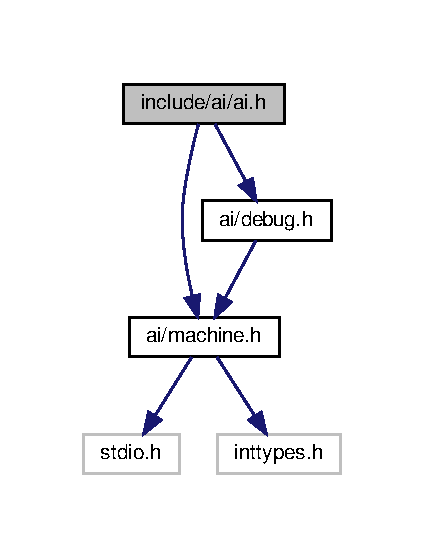
\includegraphics[width=278pt]{ai_8h__incl}
\end{center}
\end{figure}
This graph shows which files directly or indirectly include this file\+:\nopagebreak
\begin{figure}[H]
\begin{center}
\leavevmode
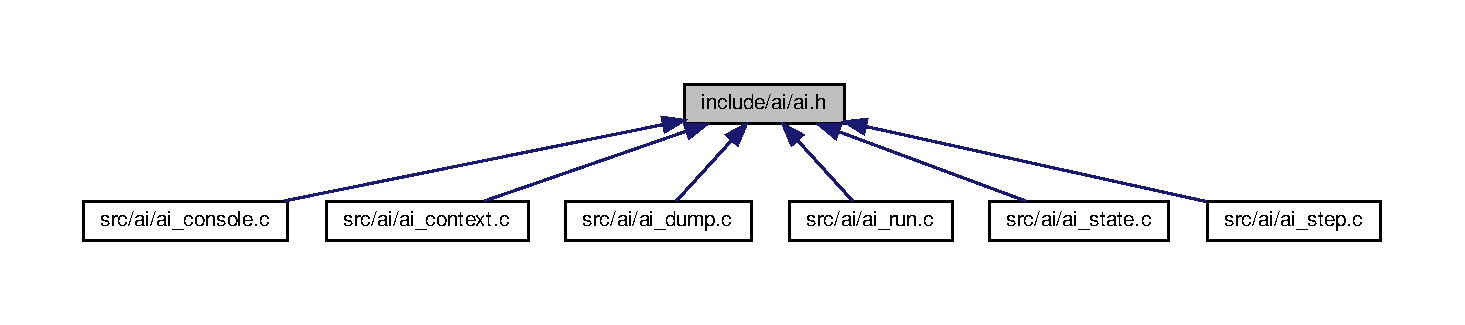
\includegraphics[width=350pt]{ai_8h__dep__incl}
\end{center}
\end{figure}


\subsection{Detailed Description}
Includes all headers of the Ases interpreter. 

\begin{DoxyAuthor}{Author}
Luiz Felipe \href{mailto:felipe.silva337@yahoo.com}{\tt felipe.\+silva337@yahoo.\+com} 
\end{DoxyAuthor}
\begin{DoxyDate}{Date}
10/2019 
\end{DoxyDate}
\begin{DoxyCopyright}{Copyright}
M\+IT License 
\end{DoxyCopyright}

\hypertarget{debug_8h}{}\section{include/ai/debug.h File Reference}
\label{debug_8h}\index{include/ai/debug.\+h@{include/ai/debug.\+h}}


Declarations about the Ases debugger.  


{\ttfamily \#include \char`\"{}ai/machine.\+h\char`\"{}}\newline
Include dependency graph for debug.\+h\+:\nopagebreak
\begin{figure}[H]
\begin{center}
\leavevmode
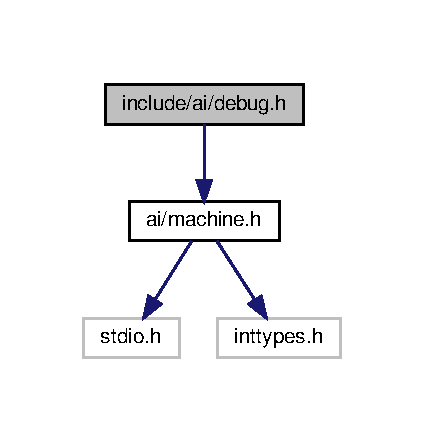
\includegraphics[width=278pt]{debug_8h__incl}
\end{center}
\end{figure}
This graph shows which files directly or indirectly include this file\+:\nopagebreak
\begin{figure}[H]
\begin{center}
\leavevmode
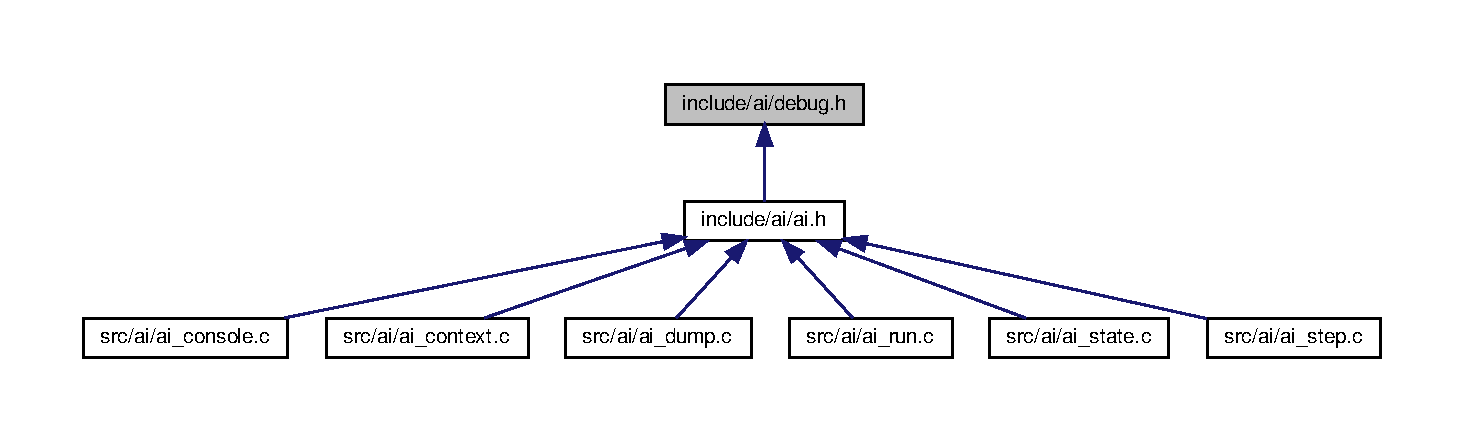
\includegraphics[width=350pt]{debug_8h__dep__incl}
\end{center}
\end{figure}
\subsection*{Functions}
\begin{DoxyCompactItemize}
\item 
void \hyperlink{debug_8h_a732b41cbc8635f8cc1aa4633df870aa1}{ai\+\_\+state} (\hyperlink{structai__machine__t}{ai\+\_\+machine\+\_\+t} $\ast$machine)
\begin{DoxyCompactList}\small\item\em Prints te state of the machine. \end{DoxyCompactList}\item 
void \hyperlink{debug_8h_a154a4b770186ba73cc1cf37ed0ffc770}{ai\+\_\+context} (\hyperlink{structai__machine__t}{ai\+\_\+machine\+\_\+t} $\ast$machine, int size)
\begin{DoxyCompactList}\small\item\em Prints the code context. \end{DoxyCompactList}\item 
void \hyperlink{debug_8h_ae34e56bcfbc3a263268d63819a87c014}{ai\+\_\+dump} (\hyperlink{structai__machine__t}{ai\+\_\+machine\+\_\+t} $\ast$machine, unsigned int start, unsigned int count)
\begin{DoxyCompactList}\small\item\em Dumps the data memory of a Ases machine. \end{DoxyCompactList}\end{DoxyCompactItemize}


\subsection{Detailed Description}
Declarations about the Ases debugger. 

\begin{DoxyAuthor}{Author}
Luiz Felipe \href{mailto:felipe.silva337@yahoo.com}{\tt felipe.\+silva337@yahoo.\+com} 
\end{DoxyAuthor}
\begin{DoxyDate}{Date}
10/2019 
\end{DoxyDate}
\begin{DoxyCopyright}{Copyright}
M\+IT License 
\end{DoxyCopyright}


\subsection{Function Documentation}
\mbox{\Hypertarget{debug_8h_a154a4b770186ba73cc1cf37ed0ffc770}\label{debug_8h_a154a4b770186ba73cc1cf37ed0ffc770}} 
\index{debug.\+h@{debug.\+h}!ai\+\_\+context@{ai\+\_\+context}}
\index{ai\+\_\+context@{ai\+\_\+context}!debug.\+h@{debug.\+h}}
\subsubsection{\texorpdfstring{ai\+\_\+context()}{ai\_context()}}
{\footnotesize\ttfamily void ai\+\_\+context (\begin{DoxyParamCaption}\item[{\hyperlink{structai__machine__t}{ai\+\_\+machine\+\_\+t} $\ast$}]{machine,  }\item[{int}]{size }\end{DoxyParamCaption})}



Prints the code context. 


\begin{DoxyParams}{Parameters}
{\em machine} & The Ases machine to print the context. \\
\hline
{\em size} & The context\textquotesingle{}s size.\\
\hline
\end{DoxyParams}
The \textquotesingle{}size\textquotesingle{} instructions left and right is printed in stdout. The current instruction is pointed with \textquotesingle{}$^\wedge$\textquotesingle{} character. \mbox{\Hypertarget{debug_8h_ae34e56bcfbc3a263268d63819a87c014}\label{debug_8h_ae34e56bcfbc3a263268d63819a87c014}} 
\index{debug.\+h@{debug.\+h}!ai\+\_\+dump@{ai\+\_\+dump}}
\index{ai\+\_\+dump@{ai\+\_\+dump}!debug.\+h@{debug.\+h}}
\subsubsection{\texorpdfstring{ai\+\_\+dump()}{ai\_dump()}}
{\footnotesize\ttfamily void ai\+\_\+dump (\begin{DoxyParamCaption}\item[{\hyperlink{structai__machine__t}{ai\+\_\+machine\+\_\+t} $\ast$}]{machine,  }\item[{unsigned int}]{start,  }\item[{unsigned int}]{count }\end{DoxyParamCaption})}



Dumps the data memory of a Ases machine. 


\begin{DoxyParams}{Parameters}
{\em machine} & The Ases machine. \\
\hline
{\em start} & The initial index to dump. \\
\hline
{\em count} & The number of elements to dump. \\
\hline
\end{DoxyParams}
\mbox{\Hypertarget{debug_8h_a732b41cbc8635f8cc1aa4633df870aa1}\label{debug_8h_a732b41cbc8635f8cc1aa4633df870aa1}} 
\index{debug.\+h@{debug.\+h}!ai\+\_\+state@{ai\+\_\+state}}
\index{ai\+\_\+state@{ai\+\_\+state}!debug.\+h@{debug.\+h}}
\subsubsection{\texorpdfstring{ai\+\_\+state()}{ai\_state()}}
{\footnotesize\ttfamily void ai\+\_\+state (\begin{DoxyParamCaption}\item[{\hyperlink{structai__machine__t}{ai\+\_\+machine\+\_\+t} $\ast$}]{machine }\end{DoxyParamCaption})}



Prints te state of the machine. 


\begin{DoxyParams}{Parameters}
{\em machine} & The Ases machine to print.\\
\hline
\end{DoxyParams}
Show the value of all the registers in hexadecimal. 
\hypertarget{machine_8h}{}\section{include/ai/machine.h File Reference}
\label{machine_8h}\index{include/ai/machine.\+h@{include/ai/machine.\+h}}


Declarations about the Ases machine.  


{\ttfamily \#include $<$stdio.\+h$>$}\newline
{\ttfamily \#include $<$inttypes.\+h$>$}\newline
Include dependency graph for machine.\+h\+:\nopagebreak
\begin{figure}[H]
\begin{center}
\leavevmode
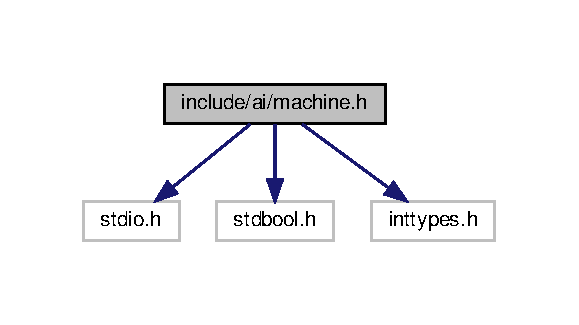
\includegraphics[width=204pt]{machine_8h__incl}
\end{center}
\end{figure}
This graph shows which files directly or indirectly include this file\+:\nopagebreak
\begin{figure}[H]
\begin{center}
\leavevmode
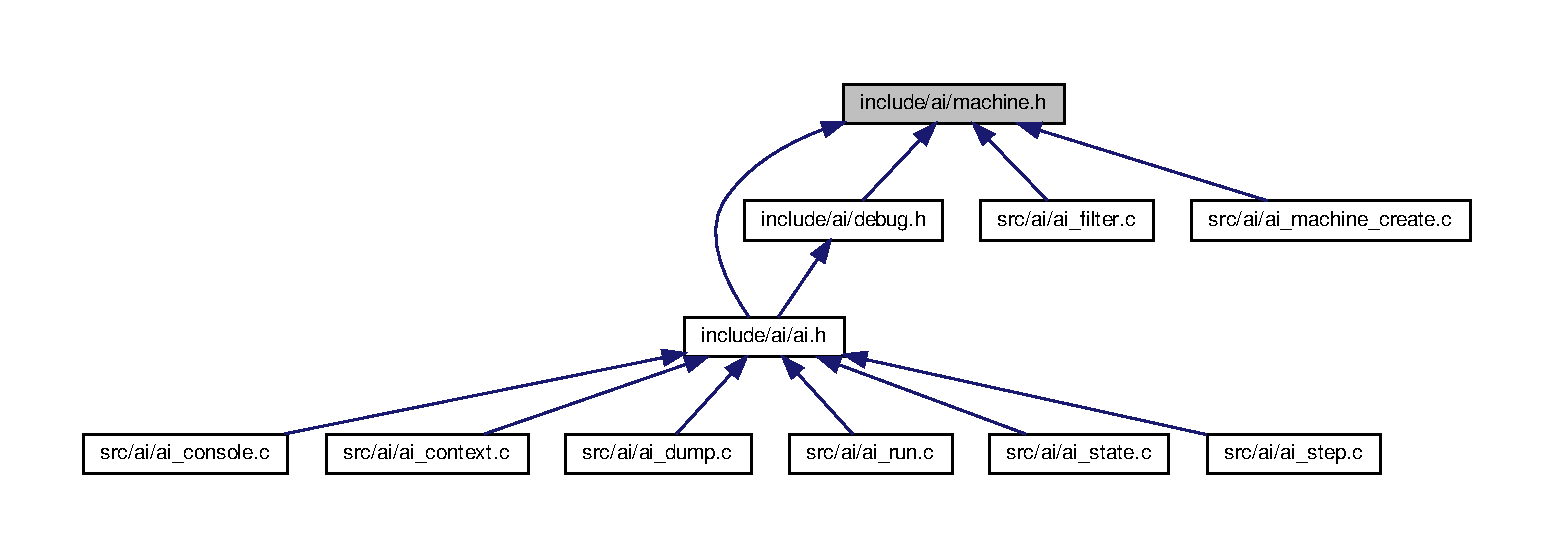
\includegraphics[width=350pt]{machine_8h__dep__incl}
\end{center}
\end{figure}
\subsection*{Data Structures}
\begin{DoxyCompactItemize}
\item 
struct \hyperlink{structai__code__t}{ai\+\_\+code\+\_\+t}
\begin{DoxyCompactList}\small\item\em Linked list for stores the instructions. \end{DoxyCompactList}\item 
struct \hyperlink{structai__machine__t}{ai\+\_\+machine\+\_\+t}
\begin{DoxyCompactList}\small\item\em Struct for stores the state of a Ases machine. \end{DoxyCompactList}\end{DoxyCompactItemize}
\subsection*{Macros}
\begin{DoxyCompactItemize}
\item 
\#define \hyperlink{machine_8h_a617e04abe8ee4d0de5f12db1afd8c344}{A\+I\+\_\+\+D\+A\+T\+A\+S\+I\+ZE}~65536
\item 
\#define \hyperlink{machine_8h_a5e27c02441546c2b9ea48e88bd57333a}{A\+I\+\_\+\+I\+N\+S\+T\+R\+U\+C\+T\+I\+O\+NS}~\char`\"{}abcd\+A\+B\+C\+Dp\+P\$$\ast$()@!=$>$$<$+-\/.?$\sim$0123456789\char`\"{}
\item 
\#define \hyperlink{machine_8h_a1ee8e54e67138dc78797dcf351366107}{A\+I\+\_\+\+C\+O\+M\+M\+E\+N\+T\+A\+RY}~\textquotesingle{}\#\textquotesingle{}
\item 
\#define \hyperlink{machine_8h_a7ed5aa79a848fccb627733031641cf45}{A\+I\+\_\+\+R\+P\+C\+O\+L\+OR}~\char`\"{}\%04\char`\"{} P\+R\+Ix16
\item 
\#define \hyperlink{machine_8h_ac9794029e3d5a153333d2d16b14a51b7}{A\+I\+\_\+\+R\+P\+R\+I\+NT}~\char`\"{}\%04\char`\"{} P\+R\+Ix16
\end{DoxyCompactItemize}
\subsection*{Typedefs}
\begin{DoxyCompactItemize}
\item 
typedef uint16\+\_\+t \hyperlink{machine_8h_a74ebfc967a5948f22ad4c9dffa32c233}{ai\+\_\+register\+\_\+t}
\end{DoxyCompactItemize}
\subsection*{Enumerations}
\begin{DoxyCompactItemize}
\item 
\mbox{\Hypertarget{machine_8h_ac2d34692cf8aa03fde6852d02d545ce5}\label{machine_8h_ac2d34692cf8aa03fde6852d02d545ce5}} 
enum \hyperlink{machine_8h_ac2d34692cf8aa03fde6852d02d545ce5}{ai\+\_\+step\+\_\+status\+\_\+t} \{ \newline
{\bfseries S\+T\+E\+P\+\_\+\+OK} = 0, 
{\bfseries S\+T\+E\+P\+\_\+\+E\+OF}, 
{\bfseries S\+T\+E\+P\+\_\+\+N\+E\+X\+T\+\_\+\+E\+OF}, 
{\bfseries S\+T\+E\+P\+\_\+\+P\+O\+I\+N\+T\+E\+R\+\_\+\+I\+N\+V\+A\+L\+ID}, 
\newline
{\bfseries S\+T\+E\+P\+\_\+\+N\+O\+T\+\_\+\+L\+M\+A\+T\+CH}, 
{\bfseries S\+T\+E\+P\+\_\+\+N\+O\+T\+\_\+\+R\+M\+A\+T\+CH}, 
{\bfseries S\+T\+E\+P\+\_\+\+D\+P\+\_\+\+O\+V\+E\+R\+F\+L\+OW}, 
{\bfseries S\+T\+E\+P\+\_\+\+D\+P\+\_\+\+U\+N\+D\+E\+R\+F\+L\+OW}, 
\newline
{\bfseries S\+T\+E\+P\+\_\+\+F\+U\+N\+C\+\_\+\+E\+R\+R\+OR}, 
{\bfseries S\+T\+E\+P\+\_\+\+F\+U\+N\+C\+\_\+\+E\+X\+IT}
 \}\begin{DoxyCompactList}\small\item\em The status returned by \hyperlink{machine_8h_aeea37f15a9edc5a9be9fc23108c41a62}{ai\+\_\+step()} function. \end{DoxyCompactList}
\end{DoxyCompactItemize}
\subsection*{Functions}
\begin{DoxyCompactItemize}
\item 
\hyperlink{structai__code__t}{ai\+\_\+code\+\_\+t} $\ast$ \hyperlink{machine_8h_af195dc53b4ff1cdc3fd61f2201c1f4c9}{ai\+\_\+filter} (F\+I\+LE $\ast$input)
\begin{DoxyCompactList}\small\item\em Filter the code and return the code. \end{DoxyCompactList}\item 
void \hyperlink{machine_8h_a849ed157f6bac41cd6cb3bfb1c1fb4ee}{ai\+\_\+code\+\_\+error} (\hyperlink{structai__code__t}{ai\+\_\+code\+\_\+t} $\ast$instruction, char $\ast$message)
\begin{DoxyCompactList}\small\item\em Prints a error message with informations about the instruction. \end{DoxyCompactList}\item 
\hyperlink{machine_8h_ac2d34692cf8aa03fde6852d02d545ce5}{ai\+\_\+step\+\_\+status\+\_\+t} \hyperlink{machine_8h_aeea37f15a9edc5a9be9fc23108c41a62}{ai\+\_\+step} (\hyperlink{structai__machine__t}{ai\+\_\+machine\+\_\+t} $\ast$machine)
\begin{DoxyCompactList}\small\item\em Run one step of the Ases machine. \end{DoxyCompactList}\item 
\hyperlink{machine_8h_ac2d34692cf8aa03fde6852d02d545ce5}{ai\+\_\+step\+\_\+status\+\_\+t} \hyperlink{machine_8h_abe076c88274d9d46f64071ad895eef38}{ai\+\_\+run} (\hyperlink{structai__machine__t}{ai\+\_\+machine\+\_\+t} $\ast$machine)
\begin{DoxyCompactList}\small\item\em Run the Ases machine while status is \textquotesingle{}S\+T\+E\+P\+\_\+\+OK\textquotesingle{}. \end{DoxyCompactList}\item 
void \hyperlink{machine_8h_afb825af073e7728de0cc879fd41c60c4}{ai\+\_\+reset} (\hyperlink{structai__machine__t}{ai\+\_\+machine\+\_\+t} $\ast$machine)
\begin{DoxyCompactList}\small\item\em Reset the Ases machine. \end{DoxyCompactList}\item 
\hyperlink{structai__machine__t}{ai\+\_\+machine\+\_\+t} $\ast$ \hyperlink{machine_8h_a32a79ad88416c4503dddaa00dd8547f6}{ai\+\_\+machine\+\_\+create} (\hyperlink{structai__code__t}{ai\+\_\+code\+\_\+t} $\ast$code)
\begin{DoxyCompactList}\small\item\em Creates a new Ases machine. \end{DoxyCompactList}\item 
void \hyperlink{machine_8h_ab12b1ee7d61cfd4173f81fea3030e626}{ai\+\_\+console} (\hyperlink{structai__machine__t}{ai\+\_\+machine\+\_\+t} $\ast$machine)
\begin{DoxyCompactList}\small\item\em Run the machine in a console debugger. \end{DoxyCompactList}\end{DoxyCompactItemize}


\subsection{Detailed Description}
Declarations about the Ases machine. 

\begin{DoxyAuthor}{Author}
Luiz Felipe \href{mailto:felipe.silva337@yahoo.com}{\tt felipe.\+silva337@yahoo.\+com} 
\end{DoxyAuthor}
\begin{DoxyDate}{Date}
10/2019 
\end{DoxyDate}
\begin{DoxyCopyright}{Copyright}
M\+IT License 
\end{DoxyCopyright}


\subsection{Macro Definition Documentation}
\mbox{\Hypertarget{machine_8h_a1ee8e54e67138dc78797dcf351366107}\label{machine_8h_a1ee8e54e67138dc78797dcf351366107}} 
\index{machine.\+h@{machine.\+h}!A\+I\+\_\+\+C\+O\+M\+M\+E\+N\+T\+A\+RY@{A\+I\+\_\+\+C\+O\+M\+M\+E\+N\+T\+A\+RY}}
\index{A\+I\+\_\+\+C\+O\+M\+M\+E\+N\+T\+A\+RY@{A\+I\+\_\+\+C\+O\+M\+M\+E\+N\+T\+A\+RY}!machine.\+h@{machine.\+h}}
\subsubsection{\texorpdfstring{A\+I\+\_\+\+C\+O\+M\+M\+E\+N\+T\+A\+RY}{AI\_COMMENTARY}}
{\footnotesize\ttfamily \#define A\+I\+\_\+\+C\+O\+M\+M\+E\+N\+T\+A\+RY~\textquotesingle{}\#\textquotesingle{}}

The character for a comentary. \mbox{\Hypertarget{machine_8h_a617e04abe8ee4d0de5f12db1afd8c344}\label{machine_8h_a617e04abe8ee4d0de5f12db1afd8c344}} 
\index{machine.\+h@{machine.\+h}!A\+I\+\_\+\+D\+A\+T\+A\+S\+I\+ZE@{A\+I\+\_\+\+D\+A\+T\+A\+S\+I\+ZE}}
\index{A\+I\+\_\+\+D\+A\+T\+A\+S\+I\+ZE@{A\+I\+\_\+\+D\+A\+T\+A\+S\+I\+ZE}!machine.\+h@{machine.\+h}}
\subsubsection{\texorpdfstring{A\+I\+\_\+\+D\+A\+T\+A\+S\+I\+ZE}{AI\_DATASIZE}}
{\footnotesize\ttfamily \#define A\+I\+\_\+\+D\+A\+T\+A\+S\+I\+ZE~65536}

The size of the data memory of a Ases machine \mbox{\Hypertarget{machine_8h_a5e27c02441546c2b9ea48e88bd57333a}\label{machine_8h_a5e27c02441546c2b9ea48e88bd57333a}} 
\index{machine.\+h@{machine.\+h}!A\+I\+\_\+\+I\+N\+S\+T\+R\+U\+C\+T\+I\+O\+NS@{A\+I\+\_\+\+I\+N\+S\+T\+R\+U\+C\+T\+I\+O\+NS}}
\index{A\+I\+\_\+\+I\+N\+S\+T\+R\+U\+C\+T\+I\+O\+NS@{A\+I\+\_\+\+I\+N\+S\+T\+R\+U\+C\+T\+I\+O\+NS}!machine.\+h@{machine.\+h}}
\subsubsection{\texorpdfstring{A\+I\+\_\+\+I\+N\+S\+T\+R\+U\+C\+T\+I\+O\+NS}{AI\_INSTRUCTIONS}}
{\footnotesize\ttfamily \#define A\+I\+\_\+\+I\+N\+S\+T\+R\+U\+C\+T\+I\+O\+NS~\char`\"{}abcd\+A\+B\+C\+Dp\+P\$$\ast$()@!=$>$$<$+-\/.?$\sim$0123456789\char`\"{}}

The list of valid instructions. \mbox{\Hypertarget{machine_8h_a7ed5aa79a848fccb627733031641cf45}\label{machine_8h_a7ed5aa79a848fccb627733031641cf45}} 
\index{machine.\+h@{machine.\+h}!A\+I\+\_\+\+R\+P\+C\+O\+L\+OR@{A\+I\+\_\+\+R\+P\+C\+O\+L\+OR}}
\index{A\+I\+\_\+\+R\+P\+C\+O\+L\+OR@{A\+I\+\_\+\+R\+P\+C\+O\+L\+OR}!machine.\+h@{machine.\+h}}
\subsubsection{\texorpdfstring{A\+I\+\_\+\+R\+P\+C\+O\+L\+OR}{AI\_RPCOLOR}}
{\footnotesize\ttfamily \#define A\+I\+\_\+\+R\+P\+C\+O\+L\+OR~\char`\"{}\%04\char`\"{} P\+R\+Ix16}

Same as A\+I\+\_\+\+R\+P\+R\+I\+NT in system is not a Unix-\/\+Like. \mbox{\Hypertarget{machine_8h_ac9794029e3d5a153333d2d16b14a51b7}\label{machine_8h_ac9794029e3d5a153333d2d16b14a51b7}} 
\index{machine.\+h@{machine.\+h}!A\+I\+\_\+\+R\+P\+R\+I\+NT@{A\+I\+\_\+\+R\+P\+R\+I\+NT}}
\index{A\+I\+\_\+\+R\+P\+R\+I\+NT@{A\+I\+\_\+\+R\+P\+R\+I\+NT}!machine.\+h@{machine.\+h}}
\subsubsection{\texorpdfstring{A\+I\+\_\+\+R\+P\+R\+I\+NT}{AI\_RPRINT}}
{\footnotesize\ttfamily \#define A\+I\+\_\+\+R\+P\+R\+I\+NT~\char`\"{}\%04\char`\"{} P\+R\+Ix16}

The format to print a register. 

\subsection{Typedef Documentation}
\mbox{\Hypertarget{machine_8h_a74ebfc967a5948f22ad4c9dffa32c233}\label{machine_8h_a74ebfc967a5948f22ad4c9dffa32c233}} 
\index{machine.\+h@{machine.\+h}!ai\+\_\+register\+\_\+t@{ai\+\_\+register\+\_\+t}}
\index{ai\+\_\+register\+\_\+t@{ai\+\_\+register\+\_\+t}!machine.\+h@{machine.\+h}}
\subsubsection{\texorpdfstring{ai\+\_\+register\+\_\+t}{ai\_register\_t}}
{\footnotesize\ttfamily typedef uint16\+\_\+t \hyperlink{machine_8h_a74ebfc967a5948f22ad4c9dffa32c233}{ai\+\_\+register\+\_\+t}}

A register in te Ases machine. 

\subsection{Function Documentation}
\mbox{\Hypertarget{machine_8h_a849ed157f6bac41cd6cb3bfb1c1fb4ee}\label{machine_8h_a849ed157f6bac41cd6cb3bfb1c1fb4ee}} 
\index{machine.\+h@{machine.\+h}!ai\+\_\+code\+\_\+error@{ai\+\_\+code\+\_\+error}}
\index{ai\+\_\+code\+\_\+error@{ai\+\_\+code\+\_\+error}!machine.\+h@{machine.\+h}}
\subsubsection{\texorpdfstring{ai\+\_\+code\+\_\+error()}{ai\_code\_error()}}
{\footnotesize\ttfamily void ai\+\_\+code\+\_\+error (\begin{DoxyParamCaption}\item[{\hyperlink{structai__code__t}{ai\+\_\+code\+\_\+t} $\ast$}]{instruction,  }\item[{char $\ast$}]{message }\end{DoxyParamCaption})}



Prints a error message with informations about the instruction. 


\begin{DoxyParams}{Parameters}
{\em instruction} & The failed instruction. \\
\hline
{\em message} & The error message to print. \\
\hline
\end{DoxyParams}
\mbox{\Hypertarget{machine_8h_ab12b1ee7d61cfd4173f81fea3030e626}\label{machine_8h_ab12b1ee7d61cfd4173f81fea3030e626}} 
\index{machine.\+h@{machine.\+h}!ai\+\_\+console@{ai\+\_\+console}}
\index{ai\+\_\+console@{ai\+\_\+console}!machine.\+h@{machine.\+h}}
\subsubsection{\texorpdfstring{ai\+\_\+console()}{ai\_console()}}
{\footnotesize\ttfamily void ai\+\_\+console (\begin{DoxyParamCaption}\item[{\hyperlink{structai__machine__t}{ai\+\_\+machine\+\_\+t} $\ast$}]{machine }\end{DoxyParamCaption})}



Run the machine in a console debugger. 


\begin{DoxyParams}{Parameters}
{\em machine} & The Ases machine. \\
\hline
\end{DoxyParams}
\mbox{\Hypertarget{machine_8h_af195dc53b4ff1cdc3fd61f2201c1f4c9}\label{machine_8h_af195dc53b4ff1cdc3fd61f2201c1f4c9}} 
\index{machine.\+h@{machine.\+h}!ai\+\_\+filter@{ai\+\_\+filter}}
\index{ai\+\_\+filter@{ai\+\_\+filter}!machine.\+h@{machine.\+h}}
\subsubsection{\texorpdfstring{ai\+\_\+filter()}{ai\_filter()}}
{\footnotesize\ttfamily \hyperlink{structai__code__t}{ai\+\_\+code\+\_\+t}$\ast$ ai\+\_\+filter (\begin{DoxyParamCaption}\item[{F\+I\+LE $\ast$}]{input }\end{DoxyParamCaption})}



Filter the code and return the code. 


\begin{DoxyParams}{Parameters}
{\em input} & The file for read the instructions \\
\hline
\end{DoxyParams}
\begin{DoxyReturn}{Returns}
The linked list to the code
\end{DoxyReturn}
Reads the instructions filtering all non-\/valid characters and removing the commentaries. Stops in the End Of File. The A\+I\+\_\+\+I\+N\+S\+T\+R\+U\+C\+T\+I\+O\+NS macro is the list of valids characters. A\+I\+\_\+\+C\+O\+M\+M\+E\+N\+T\+A\+RY is the character to one-\/line commentaries. \mbox{\Hypertarget{machine_8h_a32a79ad88416c4503dddaa00dd8547f6}\label{machine_8h_a32a79ad88416c4503dddaa00dd8547f6}} 
\index{machine.\+h@{machine.\+h}!ai\+\_\+machine\+\_\+create@{ai\+\_\+machine\+\_\+create}}
\index{ai\+\_\+machine\+\_\+create@{ai\+\_\+machine\+\_\+create}!machine.\+h@{machine.\+h}}
\subsubsection{\texorpdfstring{ai\+\_\+machine\+\_\+create()}{ai\_machine\_create()}}
{\footnotesize\ttfamily \hyperlink{structai__machine__t}{ai\+\_\+machine\+\_\+t}$\ast$ ai\+\_\+machine\+\_\+create (\begin{DoxyParamCaption}\item[{\hyperlink{structai__code__t}{ai\+\_\+code\+\_\+t} $\ast$}]{code }\end{DoxyParamCaption})}



Creates a new Ases machine. 


\begin{DoxyParams}{Parameters}
{\em code} & The code struct to the machine. \\
\hline
\end{DoxyParams}
\begin{DoxyReturn}{Returns}
The pointer to the new machine.
\end{DoxyReturn}
All the values is initialized with zero. The m-\/$>$code and m-\/$>$first is defined to the \textquotesingle{}code\textquotesingle{} argument. \mbox{\Hypertarget{machine_8h_afb825af073e7728de0cc879fd41c60c4}\label{machine_8h_afb825af073e7728de0cc879fd41c60c4}} 
\index{machine.\+h@{machine.\+h}!ai\+\_\+reset@{ai\+\_\+reset}}
\index{ai\+\_\+reset@{ai\+\_\+reset}!machine.\+h@{machine.\+h}}
\subsubsection{\texorpdfstring{ai\+\_\+reset()}{ai\_reset()}}
{\footnotesize\ttfamily void ai\+\_\+reset (\begin{DoxyParamCaption}\item[{\hyperlink{structai__machine__t}{ai\+\_\+machine\+\_\+t} $\ast$}]{machine }\end{DoxyParamCaption})}



Reset the Ases machine. 


\begin{DoxyParams}{Parameters}
{\em machine} & The Ases machine. \\
\hline
\end{DoxyParams}
\mbox{\Hypertarget{machine_8h_abe076c88274d9d46f64071ad895eef38}\label{machine_8h_abe076c88274d9d46f64071ad895eef38}} 
\index{machine.\+h@{machine.\+h}!ai\+\_\+run@{ai\+\_\+run}}
\index{ai\+\_\+run@{ai\+\_\+run}!machine.\+h@{machine.\+h}}
\subsubsection{\texorpdfstring{ai\+\_\+run()}{ai\_run()}}
{\footnotesize\ttfamily \hyperlink{machine_8h_ac2d34692cf8aa03fde6852d02d545ce5}{ai\+\_\+step\+\_\+status\+\_\+t} ai\+\_\+run (\begin{DoxyParamCaption}\item[{\hyperlink{structai__machine__t}{ai\+\_\+machine\+\_\+t} $\ast$}]{machine }\end{DoxyParamCaption})}



Run the Ases machine while status is \textquotesingle{}S\+T\+E\+P\+\_\+\+OK\textquotesingle{}. 


\begin{DoxyParams}{Parameters}
{\em machine} & The Asus machine to run. \\
\hline
\end{DoxyParams}
\mbox{\Hypertarget{machine_8h_aeea37f15a9edc5a9be9fc23108c41a62}\label{machine_8h_aeea37f15a9edc5a9be9fc23108c41a62}} 
\index{machine.\+h@{machine.\+h}!ai\+\_\+step@{ai\+\_\+step}}
\index{ai\+\_\+step@{ai\+\_\+step}!machine.\+h@{machine.\+h}}
\subsubsection{\texorpdfstring{ai\+\_\+step()}{ai\_step()}}
{\footnotesize\ttfamily \hyperlink{machine_8h_ac2d34692cf8aa03fde6852d02d545ce5}{ai\+\_\+step\+\_\+status\+\_\+t} ai\+\_\+step (\begin{DoxyParamCaption}\item[{\hyperlink{structai__machine__t}{ai\+\_\+machine\+\_\+t} $\ast$}]{machine }\end{DoxyParamCaption})}



Run one step of the Ases machine. 


\begin{DoxyParams}{Parameters}
{\em machine} & The Ases machine to run the instruction. \\
\hline
\end{DoxyParams}
\begin{DoxyReturn}{Returns}
The status of the machine. 
\end{DoxyReturn}

\hypertarget{ai__console_8c}{}\section{src/ai/ai\+\_\+console.c File Reference}
\label{ai__console_8c}\index{src/ai/ai\+\_\+console.\+c@{src/ai/ai\+\_\+console.\+c}}


The \hyperlink{ai__console_8c_ab12b1ee7d61cfd4173f81fea3030e626}{ai\+\_\+console()} source code.  


{\ttfamily \#include $<$stdio.\+h$>$}\newline
{\ttfamily \#include $<$stdbool.\+h$>$}\newline
{\ttfamily \#include \char`\"{}ai/ai.\+h\char`\"{}}\newline
Include dependency graph for ai\+\_\+console.\+c\+:
\nopagebreak
\begin{figure}[H]
\begin{center}
\leavevmode
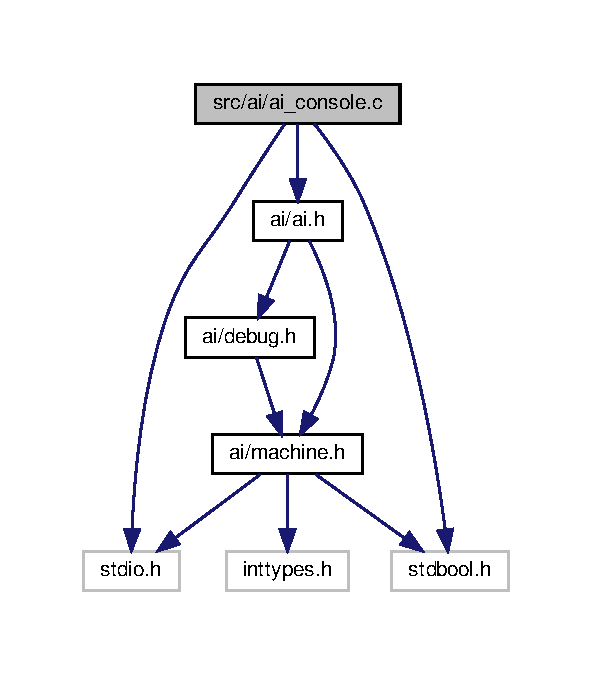
\includegraphics[width=284pt]{ai__console_8c__incl}
\end{center}
\end{figure}
\subsection*{Functions}
\begin{DoxyCompactItemize}
\item 
void \hyperlink{ai__console_8c_ab12b1ee7d61cfd4173f81fea3030e626}{ai\+\_\+console} (\hyperlink{structai__machine__t}{ai\+\_\+machine\+\_\+t} $\ast$machine)
\begin{DoxyCompactList}\small\item\em Run the machine in a console debugger. \end{DoxyCompactList}\end{DoxyCompactItemize}


\subsection{Detailed Description}
The \hyperlink{ai__console_8c_ab12b1ee7d61cfd4173f81fea3030e626}{ai\+\_\+console()} source code. 

\begin{DoxyAuthor}{Author}
Luiz Felipe \href{mailto:felipe.silva337@yahoo.com}{\tt felipe.\+silva337@yahoo.\+com} 
\end{DoxyAuthor}
\begin{DoxyDate}{Date}
10/2019 
\end{DoxyDate}
\begin{DoxyCopyright}{Copyright}
M\+IT License 
\end{DoxyCopyright}


\subsection{Function Documentation}
\mbox{\Hypertarget{ai__console_8c_ab12b1ee7d61cfd4173f81fea3030e626}\label{ai__console_8c_ab12b1ee7d61cfd4173f81fea3030e626}} 
\index{ai\+\_\+console.\+c@{ai\+\_\+console.\+c}!ai\+\_\+console@{ai\+\_\+console}}
\index{ai\+\_\+console@{ai\+\_\+console}!ai\+\_\+console.\+c@{ai\+\_\+console.\+c}}
\subsubsection{\texorpdfstring{ai\+\_\+console()}{ai\_console()}}
{\footnotesize\ttfamily void ai\+\_\+console (\begin{DoxyParamCaption}\item[{\hyperlink{structai__machine__t}{ai\+\_\+machine\+\_\+t} $\ast$}]{machine }\end{DoxyParamCaption})}



Run the machine in a console debugger. 


\begin{DoxyParams}{Parameters}
{\em machine} & The Ases machine. \\
\hline
\end{DoxyParams}

\hypertarget{ai__context_8c}{}\section{src/ai/ai\+\_\+context.c File Reference}
\label{ai__context_8c}\index{src/ai/ai\+\_\+context.\+c@{src/ai/ai\+\_\+context.\+c}}


The \hyperlink{ai__context_8c_a154a4b770186ba73cc1cf37ed0ffc770}{ai\+\_\+context()} source code.  


{\ttfamily \#include \char`\"{}ai/ai.\+h\char`\"{}}\newline
Include dependency graph for ai\+\_\+context.\+c\+:
\nopagebreak
\begin{figure}[H]
\begin{center}
\leavevmode
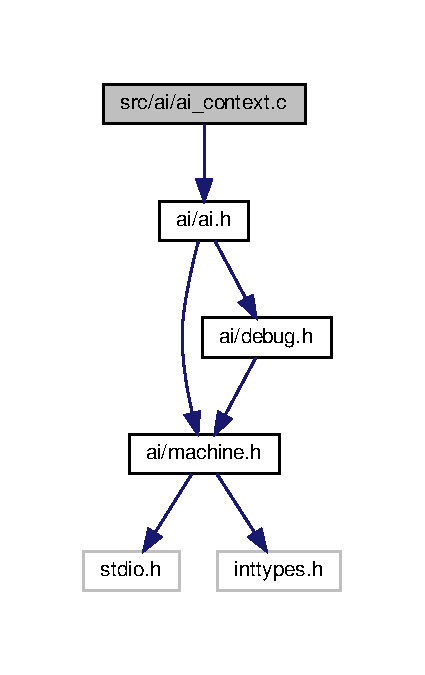
\includegraphics[width=278pt]{ai__context_8c__incl}
\end{center}
\end{figure}
\subsection*{Functions}
\begin{DoxyCompactItemize}
\item 
void \hyperlink{ai__context_8c_a154a4b770186ba73cc1cf37ed0ffc770}{ai\+\_\+context} (\hyperlink{structai__machine__t}{ai\+\_\+machine\+\_\+t} $\ast$machine, int size)
\begin{DoxyCompactList}\small\item\em Prints the code context. \end{DoxyCompactList}\end{DoxyCompactItemize}


\subsection{Detailed Description}
The \hyperlink{ai__context_8c_a154a4b770186ba73cc1cf37ed0ffc770}{ai\+\_\+context()} source code. 

\begin{DoxyAuthor}{Author}
Luiz Felipe \href{mailto:felipe.silva337@yahoo.com}{\tt felipe.\+silva337@yahoo.\+com} 
\end{DoxyAuthor}
\begin{DoxyDate}{Date}
10/2019 
\end{DoxyDate}
\begin{DoxyCopyright}{Copyright}
M\+IT License 
\end{DoxyCopyright}


\subsection{Function Documentation}
\mbox{\Hypertarget{ai__context_8c_a154a4b770186ba73cc1cf37ed0ffc770}\label{ai__context_8c_a154a4b770186ba73cc1cf37ed0ffc770}} 
\index{ai\+\_\+context.\+c@{ai\+\_\+context.\+c}!ai\+\_\+context@{ai\+\_\+context}}
\index{ai\+\_\+context@{ai\+\_\+context}!ai\+\_\+context.\+c@{ai\+\_\+context.\+c}}
\subsubsection{\texorpdfstring{ai\+\_\+context()}{ai\_context()}}
{\footnotesize\ttfamily void ai\+\_\+context (\begin{DoxyParamCaption}\item[{\hyperlink{structai__machine__t}{ai\+\_\+machine\+\_\+t} $\ast$}]{machine,  }\item[{int}]{size }\end{DoxyParamCaption})}



Prints the code context. 


\begin{DoxyParams}{Parameters}
{\em machine} & The Ases machine to print the context. \\
\hline
{\em size} & The context\textquotesingle{}s size.\\
\hline
\end{DoxyParams}
The \textquotesingle{}size\textquotesingle{} instructions left and right is printed in stdout. The current instruction is pointed with \textquotesingle{}$^\wedge$\textquotesingle{} character. 
\hypertarget{ai__dump_8c}{}\section{src/ai/ai\+\_\+dump.c File Reference}
\label{ai__dump_8c}\index{src/ai/ai\+\_\+dump.\+c@{src/ai/ai\+\_\+dump.\+c}}


The \hyperlink{ai__dump_8c_ae34e56bcfbc3a263268d63819a87c014}{ai\+\_\+dump()} source code.  


{\ttfamily \#include \char`\"{}ai/ai.\+h\char`\"{}}\newline
Include dependency graph for ai\+\_\+dump.\+c\+:
\nopagebreak
\begin{figure}[H]
\begin{center}
\leavevmode
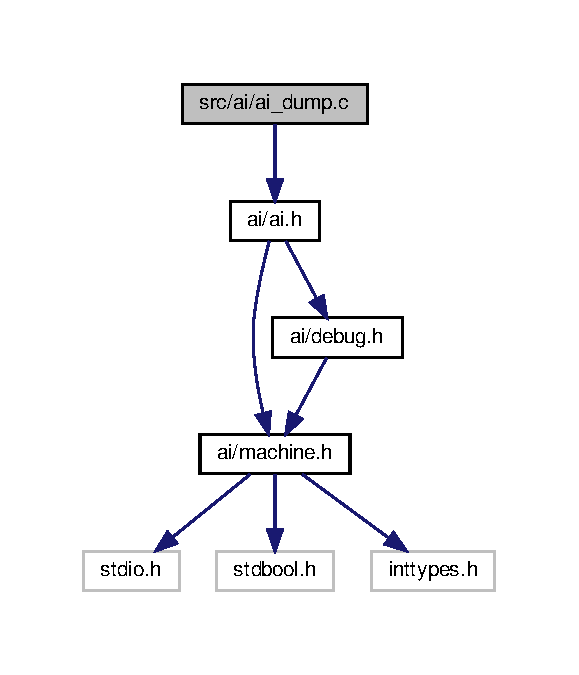
\includegraphics[width=278pt]{ai__dump_8c__incl}
\end{center}
\end{figure}
\subsection*{Functions}
\begin{DoxyCompactItemize}
\item 
void \hyperlink{ai__dump_8c_ae34e56bcfbc3a263268d63819a87c014}{ai\+\_\+dump} (\hyperlink{structai__machine__t}{ai\+\_\+machine\+\_\+t} $\ast$machine, unsigned int start, unsigned int count)
\begin{DoxyCompactList}\small\item\em Dumps the data memory of a Ases machine. \end{DoxyCompactList}\end{DoxyCompactItemize}


\subsection{Detailed Description}
The \hyperlink{ai__dump_8c_ae34e56bcfbc3a263268d63819a87c014}{ai\+\_\+dump()} source code. 

\begin{DoxyAuthor}{Author}
Luiz Felipe \href{mailto:felipe.silva337@yahoo.com}{\tt felipe.\+silva337@yahoo.\+com} 
\end{DoxyAuthor}
\begin{DoxyDate}{Date}
10/2019 
\end{DoxyDate}
\begin{DoxyCopyright}{Copyright}
M\+IT License 
\end{DoxyCopyright}


\subsection{Function Documentation}
\mbox{\Hypertarget{ai__dump_8c_ae34e56bcfbc3a263268d63819a87c014}\label{ai__dump_8c_ae34e56bcfbc3a263268d63819a87c014}} 
\index{ai\+\_\+dump.\+c@{ai\+\_\+dump.\+c}!ai\+\_\+dump@{ai\+\_\+dump}}
\index{ai\+\_\+dump@{ai\+\_\+dump}!ai\+\_\+dump.\+c@{ai\+\_\+dump.\+c}}
\subsubsection{\texorpdfstring{ai\+\_\+dump()}{ai\_dump()}}
{\footnotesize\ttfamily void ai\+\_\+dump (\begin{DoxyParamCaption}\item[{\hyperlink{structai__machine__t}{ai\+\_\+machine\+\_\+t} $\ast$}]{machine,  }\item[{unsigned int}]{start,  }\item[{unsigned int}]{count }\end{DoxyParamCaption})}



Dumps the data memory of a Ases machine. 


\begin{DoxyParams}{Parameters}
{\em machine} & The Ases machine. \\
\hline
{\em start} & The initial index to dump. \\
\hline
{\em count} & The number of elements to dump. \\
\hline
\end{DoxyParams}

\hypertarget{ai__filter_8c}{}\section{src/ai/ai\+\_\+filter.c File Reference}
\label{ai__filter_8c}\index{src/ai/ai\+\_\+filter.\+c@{src/ai/ai\+\_\+filter.\+c}}


The \hyperlink{ai__filter_8c_af195dc53b4ff1cdc3fd61f2201c1f4c9}{ai\+\_\+filter()} source code.  


{\ttfamily \#include $<$stdlib.\+h$>$}\newline
{\ttfamily \#include $<$stdbool.\+h$>$}\newline
{\ttfamily \#include $<$string.\+h$>$}\newline
{\ttfamily \#include \char`\"{}ai/machine.\+h\char`\"{}}\newline
Include dependency graph for ai\+\_\+filter.\+c\+:\nopagebreak
\begin{figure}[H]
\begin{center}
\leavevmode
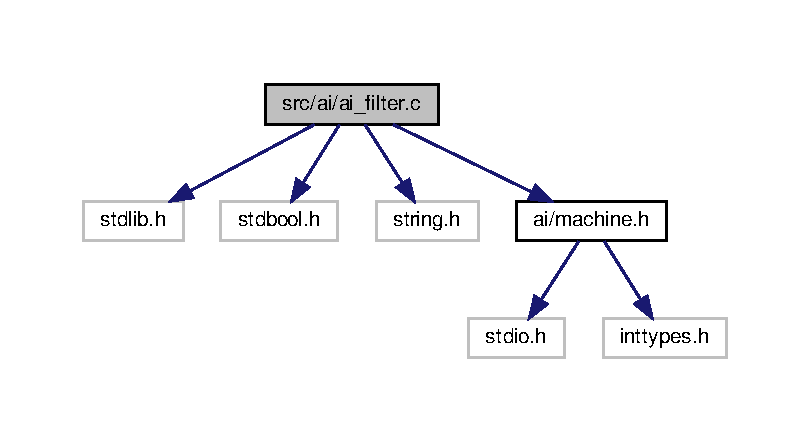
\includegraphics[width=350pt]{ai__filter_8c__incl}
\end{center}
\end{figure}
\subsection*{Functions}
\begin{DoxyCompactItemize}
\item 
\hyperlink{structai__code__t}{ai\+\_\+code\+\_\+t} $\ast$ \hyperlink{ai__filter_8c_af195dc53b4ff1cdc3fd61f2201c1f4c9}{ai\+\_\+filter} (F\+I\+LE $\ast$input)
\begin{DoxyCompactList}\small\item\em Filter the code and return the code. \end{DoxyCompactList}\end{DoxyCompactItemize}


\subsection{Detailed Description}
The \hyperlink{ai__filter_8c_af195dc53b4ff1cdc3fd61f2201c1f4c9}{ai\+\_\+filter()} source code. 

\begin{DoxyAuthor}{Author}
Luiz Felipe \href{mailto:felipe.silva337@yahoo.com}{\tt felipe.\+silva337@yahoo.\+com} 
\end{DoxyAuthor}
\begin{DoxyDate}{Date}
10/2019 
\end{DoxyDate}
\begin{DoxyCopyright}{Copyright}
M\+IT License 
\end{DoxyCopyright}


\subsection{Function Documentation}
\mbox{\Hypertarget{ai__filter_8c_af195dc53b4ff1cdc3fd61f2201c1f4c9}\label{ai__filter_8c_af195dc53b4ff1cdc3fd61f2201c1f4c9}} 
\index{ai\+\_\+filter.\+c@{ai\+\_\+filter.\+c}!ai\+\_\+filter@{ai\+\_\+filter}}
\index{ai\+\_\+filter@{ai\+\_\+filter}!ai\+\_\+filter.\+c@{ai\+\_\+filter.\+c}}
\subsubsection{\texorpdfstring{ai\+\_\+filter()}{ai\_filter()}}
{\footnotesize\ttfamily \hyperlink{structai__code__t}{ai\+\_\+code\+\_\+t}$\ast$ ai\+\_\+filter (\begin{DoxyParamCaption}\item[{F\+I\+LE $\ast$}]{input }\end{DoxyParamCaption})}



Filter the code and return the code. 


\begin{DoxyParams}{Parameters}
{\em input} & The file for read the instructions \\
\hline
\end{DoxyParams}
\begin{DoxyReturn}{Returns}
The linked list to the code
\end{DoxyReturn}
Reads the instructions filtering all non-\/valid characters and removing the commentaries. Stops in the End Of File. The A\+I\+\_\+\+I\+N\+S\+T\+R\+U\+C\+T\+I\+O\+NS macro is the list of valids characters. A\+I\+\_\+\+C\+O\+M\+M\+E\+N\+T\+A\+RY is the character to one-\/line commentaries. 
\hypertarget{ai__machine__create_8c}{}\section{src/ai/ai\+\_\+machine\+\_\+create.c File Reference}
\label{ai__machine__create_8c}\index{src/ai/ai\+\_\+machine\+\_\+create.\+c@{src/ai/ai\+\_\+machine\+\_\+create.\+c}}


The \hyperlink{ai__machine__create_8c_a32a79ad88416c4503dddaa00dd8547f6}{ai\+\_\+machine\+\_\+create()} source code.  


{\ttfamily \#include $<$stdlib.\+h$>$}\newline
{\ttfamily \#include \char`\"{}ai/machine.\+h\char`\"{}}\newline
Include dependency graph for ai\+\_\+machine\+\_\+create.\+c\+:\nopagebreak
\begin{figure}[H]
\begin{center}
\leavevmode
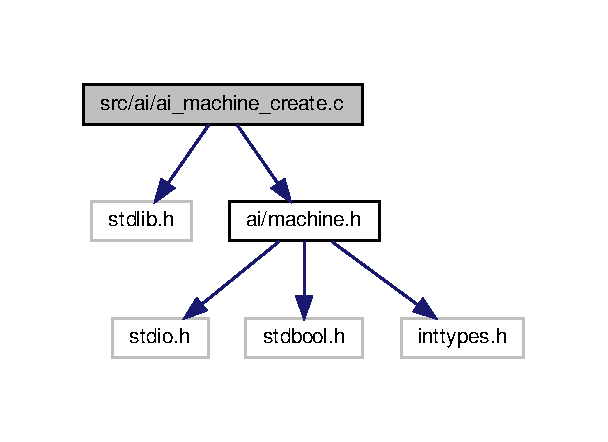
\includegraphics[width=251pt]{ai__machine__create_8c__incl}
\end{center}
\end{figure}
\subsection*{Functions}
\begin{DoxyCompactItemize}
\item 
\hyperlink{structai__machine__t}{ai\+\_\+machine\+\_\+t} $\ast$ \hyperlink{ai__machine__create_8c_a32a79ad88416c4503dddaa00dd8547f6}{ai\+\_\+machine\+\_\+create} (\hyperlink{structai__code__t}{ai\+\_\+code\+\_\+t} $\ast$code)
\begin{DoxyCompactList}\small\item\em Creates a new Ases machine. \end{DoxyCompactList}\end{DoxyCompactItemize}


\subsection{Detailed Description}
The \hyperlink{ai__machine__create_8c_a32a79ad88416c4503dddaa00dd8547f6}{ai\+\_\+machine\+\_\+create()} source code. 

\begin{DoxyAuthor}{Author}
Luiz Felipe \href{mailto:felipe.silva337@yahoo.com}{\tt felipe.\+silva337@yahoo.\+com} 
\end{DoxyAuthor}
\begin{DoxyDate}{Date}
10/2019 
\end{DoxyDate}
\begin{DoxyCopyright}{Copyright}
M\+IT License 
\end{DoxyCopyright}


\subsection{Function Documentation}
\mbox{\Hypertarget{ai__machine__create_8c_a32a79ad88416c4503dddaa00dd8547f6}\label{ai__machine__create_8c_a32a79ad88416c4503dddaa00dd8547f6}} 
\index{ai\+\_\+machine\+\_\+create.\+c@{ai\+\_\+machine\+\_\+create.\+c}!ai\+\_\+machine\+\_\+create@{ai\+\_\+machine\+\_\+create}}
\index{ai\+\_\+machine\+\_\+create@{ai\+\_\+machine\+\_\+create}!ai\+\_\+machine\+\_\+create.\+c@{ai\+\_\+machine\+\_\+create.\+c}}
\subsubsection{\texorpdfstring{ai\+\_\+machine\+\_\+create()}{ai\_machine\_create()}}
{\footnotesize\ttfamily \hyperlink{structai__machine__t}{ai\+\_\+machine\+\_\+t}$\ast$ ai\+\_\+machine\+\_\+create (\begin{DoxyParamCaption}\item[{\hyperlink{structai__code__t}{ai\+\_\+code\+\_\+t} $\ast$}]{code }\end{DoxyParamCaption})}



Creates a new Ases machine. 


\begin{DoxyParams}{Parameters}
{\em code} & The code struct to the machine. \\
\hline
\end{DoxyParams}
\begin{DoxyReturn}{Returns}
The pointer to the new machine.
\end{DoxyReturn}
All the values is initialized with zero. The m-\/$>$code and m-\/$>$first is defined to the \textquotesingle{}code\textquotesingle{} argument. 
\hypertarget{ai__run_8c}{}\section{src/ai/ai\+\_\+run.c File Reference}
\label{ai__run_8c}\index{src/ai/ai\+\_\+run.\+c@{src/ai/ai\+\_\+run.\+c}}


The \hyperlink{ai__run_8c_abe076c88274d9d46f64071ad895eef38}{ai\+\_\+run()} and \hyperlink{ai__run_8c_afb825af073e7728de0cc879fd41c60c4}{ai\+\_\+reset()} source code.  


{\ttfamily \#include $<$string.\+h$>$}\newline
{\ttfamily \#include \char`\"{}ai/ai.\+h\char`\"{}}\newline
Include dependency graph for ai\+\_\+run.\+c\+:
\nopagebreak
\begin{figure}[H]
\begin{center}
\leavevmode
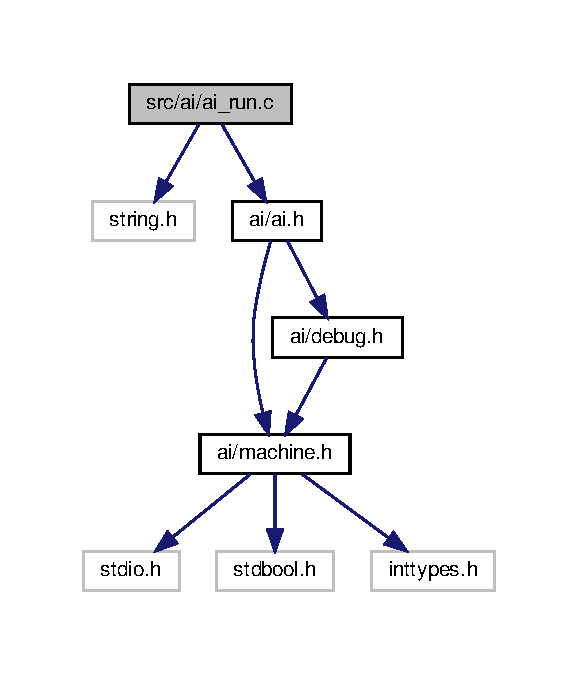
\includegraphics[width=278pt]{ai__run_8c__incl}
\end{center}
\end{figure}
\subsection*{Functions}
\begin{DoxyCompactItemize}
\item 
\hyperlink{machine_8h_ac2d34692cf8aa03fde6852d02d545ce5}{ai\+\_\+step\+\_\+status\+\_\+t} \hyperlink{ai__run_8c_abe076c88274d9d46f64071ad895eef38}{ai\+\_\+run} (\hyperlink{structai__machine__t}{ai\+\_\+machine\+\_\+t} $\ast$machine)
\begin{DoxyCompactList}\small\item\em Run the Ases machine while status is \textquotesingle{}S\+T\+E\+P\+\_\+\+OK\textquotesingle{}. \end{DoxyCompactList}\item 
void \hyperlink{ai__run_8c_afb825af073e7728de0cc879fd41c60c4}{ai\+\_\+reset} (\hyperlink{structai__machine__t}{ai\+\_\+machine\+\_\+t} $\ast$machine)
\begin{DoxyCompactList}\small\item\em Reset the Ases machine. \end{DoxyCompactList}\end{DoxyCompactItemize}


\subsection{Detailed Description}
The \hyperlink{ai__run_8c_abe076c88274d9d46f64071ad895eef38}{ai\+\_\+run()} and \hyperlink{ai__run_8c_afb825af073e7728de0cc879fd41c60c4}{ai\+\_\+reset()} source code. 

\begin{DoxyAuthor}{Author}
Luiz Felipe \href{mailto:felipe.silva337@yahoo.com}{\tt felipe.\+silva337@yahoo.\+com} 
\end{DoxyAuthor}
\begin{DoxyDate}{Date}
10/2019 
\end{DoxyDate}
\begin{DoxyCopyright}{Copyright}
M\+IT License 
\end{DoxyCopyright}


\subsection{Function Documentation}
\mbox{\Hypertarget{ai__run_8c_afb825af073e7728de0cc879fd41c60c4}\label{ai__run_8c_afb825af073e7728de0cc879fd41c60c4}} 
\index{ai\+\_\+run.\+c@{ai\+\_\+run.\+c}!ai\+\_\+reset@{ai\+\_\+reset}}
\index{ai\+\_\+reset@{ai\+\_\+reset}!ai\+\_\+run.\+c@{ai\+\_\+run.\+c}}
\subsubsection{\texorpdfstring{ai\+\_\+reset()}{ai\_reset()}}
{\footnotesize\ttfamily void ai\+\_\+reset (\begin{DoxyParamCaption}\item[{\hyperlink{structai__machine__t}{ai\+\_\+machine\+\_\+t} $\ast$}]{machine }\end{DoxyParamCaption})}



Reset the Ases machine. 


\begin{DoxyParams}{Parameters}
{\em machine} & The Ases machine. \\
\hline
\end{DoxyParams}
\mbox{\Hypertarget{ai__run_8c_abe076c88274d9d46f64071ad895eef38}\label{ai__run_8c_abe076c88274d9d46f64071ad895eef38}} 
\index{ai\+\_\+run.\+c@{ai\+\_\+run.\+c}!ai\+\_\+run@{ai\+\_\+run}}
\index{ai\+\_\+run@{ai\+\_\+run}!ai\+\_\+run.\+c@{ai\+\_\+run.\+c}}
\subsubsection{\texorpdfstring{ai\+\_\+run()}{ai\_run()}}
{\footnotesize\ttfamily \hyperlink{machine_8h_ac2d34692cf8aa03fde6852d02d545ce5}{ai\+\_\+step\+\_\+status\+\_\+t} ai\+\_\+run (\begin{DoxyParamCaption}\item[{\hyperlink{structai__machine__t}{ai\+\_\+machine\+\_\+t} $\ast$}]{machine }\end{DoxyParamCaption})}



Run the Ases machine while status is \textquotesingle{}S\+T\+E\+P\+\_\+\+OK\textquotesingle{}. 


\begin{DoxyParams}{Parameters}
{\em machine} & The Asus machine to run. \\
\hline
\end{DoxyParams}

\hypertarget{ai__state_8c}{}\section{src/ai/ai\+\_\+state.c File Reference}
\label{ai__state_8c}\index{src/ai/ai\+\_\+state.\+c@{src/ai/ai\+\_\+state.\+c}}


The \hyperlink{ai__state_8c_a732b41cbc8635f8cc1aa4633df870aa1}{ai\+\_\+state()} source code.  


{\ttfamily \#include \char`\"{}ai/ai.\+h\char`\"{}}\newline
Include dependency graph for ai\+\_\+state.\+c\+:\nopagebreak
\begin{figure}[H]
\begin{center}
\leavevmode
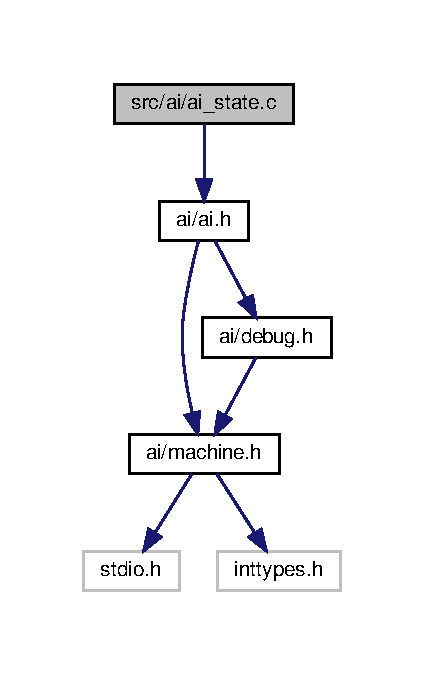
\includegraphics[width=204pt]{ai__state_8c__incl}
\end{center}
\end{figure}
\subsection*{Functions}
\begin{DoxyCompactItemize}
\item 
void \hyperlink{ai__state_8c_a732b41cbc8635f8cc1aa4633df870aa1}{ai\+\_\+state} (\hyperlink{structai__machine__t}{ai\+\_\+machine\+\_\+t} $\ast$machine)
\begin{DoxyCompactList}\small\item\em Prints te state of the machine. \end{DoxyCompactList}\end{DoxyCompactItemize}


\subsection{Detailed Description}
The \hyperlink{ai__state_8c_a732b41cbc8635f8cc1aa4633df870aa1}{ai\+\_\+state()} source code. 

\begin{DoxyAuthor}{Author}
Luiz Felipe \href{mailto:felipe.silva337@yahoo.com}{\tt felipe.\+silva337@yahoo.\+com} 
\end{DoxyAuthor}
\begin{DoxyDate}{Date}
10/2019 
\end{DoxyDate}
\begin{DoxyCopyright}{Copyright}
M\+IT License 
\end{DoxyCopyright}


\subsection{Function Documentation}
\mbox{\Hypertarget{ai__state_8c_a732b41cbc8635f8cc1aa4633df870aa1}\label{ai__state_8c_a732b41cbc8635f8cc1aa4633df870aa1}} 
\index{ai\+\_\+state.\+c@{ai\+\_\+state.\+c}!ai\+\_\+state@{ai\+\_\+state}}
\index{ai\+\_\+state@{ai\+\_\+state}!ai\+\_\+state.\+c@{ai\+\_\+state.\+c}}
\subsubsection{\texorpdfstring{ai\+\_\+state()}{ai\_state()}}
{\footnotesize\ttfamily void ai\+\_\+state (\begin{DoxyParamCaption}\item[{\hyperlink{structai__machine__t}{ai\+\_\+machine\+\_\+t} $\ast$}]{machine }\end{DoxyParamCaption})}



Prints te state of the machine. 


\begin{DoxyParams}{Parameters}
{\em machine} & The Ases machine to print.\\
\hline
\end{DoxyParams}
Show the value of all the registers in hexadecimal. 
\hypertarget{ai__step_8c}{}\section{src/ai/ai\+\_\+step.c File Reference}
\label{ai__step_8c}\index{src/ai/ai\+\_\+step.\+c@{src/ai/ai\+\_\+step.\+c}}


The \hyperlink{ai__step_8c_aeea37f15a9edc5a9be9fc23108c41a62}{ai\+\_\+step()}, \hyperlink{ai__step_8c_ae3cfcf99aa5a6889a67d2c8cf1e0fbfc}{ai\+\_\+code\+\_\+sindex()}, \hyperlink{ai__step_8c_a4e5c597b7363ec64f152df5779857bfc}{ai\+\_\+code\+\_\+smatch()} and \hyperlink{ai__step_8c_a849ed157f6bac41cd6cb3bfb1c1fb4ee}{ai\+\_\+code\+\_\+error()} source code.  


{\ttfamily \#include $<$stdlib.\+h$>$}\newline
{\ttfamily \#include \char`\"{}ai/ai.\+h\char`\"{}}\newline
Include dependency graph for ai\+\_\+step.\+c\+:
\nopagebreak
\begin{figure}[H]
\begin{center}
\leavevmode
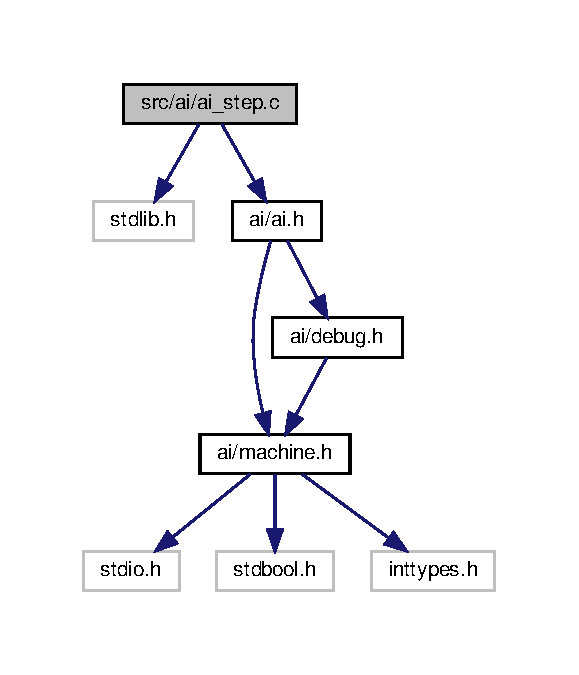
\includegraphics[width=278pt]{ai__step_8c__incl}
\end{center}
\end{figure}
\subsection*{Functions}
\begin{DoxyCompactItemize}
\item 
\hyperlink{structai__code__t}{ai\+\_\+code\+\_\+t} $\ast$ \hyperlink{ai__step_8c_ae3cfcf99aa5a6889a67d2c8cf1e0fbfc}{ai\+\_\+code\+\_\+sindex} (\hyperlink{structai__code__t}{ai\+\_\+code\+\_\+t} $\ast$code, int index)
\begin{DoxyCompactList}\small\item\em Search for a instruction by the index. \end{DoxyCompactList}\item 
\hyperlink{structai__code__t}{ai\+\_\+code\+\_\+t} $\ast$ \hyperlink{ai__step_8c_a4e5c597b7363ec64f152df5779857bfc}{ai\+\_\+code\+\_\+smatch} (\hyperlink{structai__code__t}{ai\+\_\+code\+\_\+t} $\ast$code, char direction)
\begin{DoxyCompactList}\small\item\em Search for matched \textquotesingle{}@\textquotesingle{} for left or right. \end{DoxyCompactList}\item 
void \hyperlink{ai__step_8c_a849ed157f6bac41cd6cb3bfb1c1fb4ee}{ai\+\_\+code\+\_\+error} (\hyperlink{structai__code__t}{ai\+\_\+code\+\_\+t} $\ast$instruction, char $\ast$message)
\begin{DoxyCompactList}\small\item\em Prints a error message with informations about the instruction. \end{DoxyCompactList}\item 
\hyperlink{machine_8h_ac2d34692cf8aa03fde6852d02d545ce5}{ai\+\_\+step\+\_\+status\+\_\+t} \hyperlink{ai__step_8c_aeea37f15a9edc5a9be9fc23108c41a62}{ai\+\_\+step} (\hyperlink{structai__machine__t}{ai\+\_\+machine\+\_\+t} $\ast$machine)
\begin{DoxyCompactList}\small\item\em Run one step of the Ases machine. \end{DoxyCompactList}\end{DoxyCompactItemize}


\subsection{Detailed Description}
The \hyperlink{ai__step_8c_aeea37f15a9edc5a9be9fc23108c41a62}{ai\+\_\+step()}, \hyperlink{ai__step_8c_ae3cfcf99aa5a6889a67d2c8cf1e0fbfc}{ai\+\_\+code\+\_\+sindex()}, \hyperlink{ai__step_8c_a4e5c597b7363ec64f152df5779857bfc}{ai\+\_\+code\+\_\+smatch()} and \hyperlink{ai__step_8c_a849ed157f6bac41cd6cb3bfb1c1fb4ee}{ai\+\_\+code\+\_\+error()} source code. 

\begin{DoxyAuthor}{Author}
Luiz Felipe \href{mailto:felipe.silva337@yahoo.com}{\tt felipe.\+silva337@yahoo.\+com} 
\end{DoxyAuthor}
\begin{DoxyDate}{Date}
10/2019 
\end{DoxyDate}
\begin{DoxyCopyright}{Copyright}
M\+IT License 
\end{DoxyCopyright}


\subsection{Function Documentation}
\mbox{\Hypertarget{ai__step_8c_a849ed157f6bac41cd6cb3bfb1c1fb4ee}\label{ai__step_8c_a849ed157f6bac41cd6cb3bfb1c1fb4ee}} 
\index{ai\+\_\+step.\+c@{ai\+\_\+step.\+c}!ai\+\_\+code\+\_\+error@{ai\+\_\+code\+\_\+error}}
\index{ai\+\_\+code\+\_\+error@{ai\+\_\+code\+\_\+error}!ai\+\_\+step.\+c@{ai\+\_\+step.\+c}}
\subsubsection{\texorpdfstring{ai\+\_\+code\+\_\+error()}{ai\_code\_error()}}
{\footnotesize\ttfamily void ai\+\_\+code\+\_\+error (\begin{DoxyParamCaption}\item[{\hyperlink{structai__code__t}{ai\+\_\+code\+\_\+t} $\ast$}]{instruction,  }\item[{char $\ast$}]{message }\end{DoxyParamCaption})}



Prints a error message with informations about the instruction. 


\begin{DoxyParams}{Parameters}
{\em instruction} & The failed instruction. \\
\hline
{\em message} & The error message to print. \\
\hline
\end{DoxyParams}
\mbox{\Hypertarget{ai__step_8c_ae3cfcf99aa5a6889a67d2c8cf1e0fbfc}\label{ai__step_8c_ae3cfcf99aa5a6889a67d2c8cf1e0fbfc}} 
\index{ai\+\_\+step.\+c@{ai\+\_\+step.\+c}!ai\+\_\+code\+\_\+sindex@{ai\+\_\+code\+\_\+sindex}}
\index{ai\+\_\+code\+\_\+sindex@{ai\+\_\+code\+\_\+sindex}!ai\+\_\+step.\+c@{ai\+\_\+step.\+c}}
\subsubsection{\texorpdfstring{ai\+\_\+code\+\_\+sindex()}{ai\_code\_sindex()}}
{\footnotesize\ttfamily \hyperlink{structai__code__t}{ai\+\_\+code\+\_\+t}$\ast$ ai\+\_\+code\+\_\+sindex (\begin{DoxyParamCaption}\item[{\hyperlink{structai__code__t}{ai\+\_\+code\+\_\+t} $\ast$}]{code,  }\item[{int}]{index }\end{DoxyParamCaption})}



Search for a instruction by the index. 


\begin{DoxyParams}{Parameters}
{\em code} & The code struct. \\
\hline
{\em index} & The index of the instruction to search. \\
\hline
\end{DoxyParams}

\begin{DoxyRetVals}{Return values}
{\em N\+U\+LL} & If not find the instruction. \\
\hline
\end{DoxyRetVals}
\begin{DoxyReturn}{Returns}
The pointer to the instruction. 
\end{DoxyReturn}
\mbox{\Hypertarget{ai__step_8c_a4e5c597b7363ec64f152df5779857bfc}\label{ai__step_8c_a4e5c597b7363ec64f152df5779857bfc}} 
\index{ai\+\_\+step.\+c@{ai\+\_\+step.\+c}!ai\+\_\+code\+\_\+smatch@{ai\+\_\+code\+\_\+smatch}}
\index{ai\+\_\+code\+\_\+smatch@{ai\+\_\+code\+\_\+smatch}!ai\+\_\+step.\+c@{ai\+\_\+step.\+c}}
\subsubsection{\texorpdfstring{ai\+\_\+code\+\_\+smatch()}{ai\_code\_smatch()}}
{\footnotesize\ttfamily \hyperlink{structai__code__t}{ai\+\_\+code\+\_\+t}$\ast$ ai\+\_\+code\+\_\+smatch (\begin{DoxyParamCaption}\item[{\hyperlink{structai__code__t}{ai\+\_\+code\+\_\+t} $\ast$}]{code,  }\item[{char}]{direction }\end{DoxyParamCaption})}



Search for matched \textquotesingle{}@\textquotesingle{} for left or right. 


\begin{DoxyParams}{Parameters}
{\em code} & The initial instruction. \\
\hline
{\em direction} & \textquotesingle{}L\textquotesingle{} to left, \textquotesingle{}R\textquotesingle{} to right. \\
\hline
\end{DoxyParams}

\begin{DoxyRetVals}{Return values}
{\em N\+U\+LL} & If not matched any instruction. \\
\hline
\end{DoxyRetVals}
\begin{DoxyReturn}{Returns}
The matched instruction. 
\end{DoxyReturn}
\mbox{\Hypertarget{ai__step_8c_aeea37f15a9edc5a9be9fc23108c41a62}\label{ai__step_8c_aeea37f15a9edc5a9be9fc23108c41a62}} 
\index{ai\+\_\+step.\+c@{ai\+\_\+step.\+c}!ai\+\_\+step@{ai\+\_\+step}}
\index{ai\+\_\+step@{ai\+\_\+step}!ai\+\_\+step.\+c@{ai\+\_\+step.\+c}}
\subsubsection{\texorpdfstring{ai\+\_\+step()}{ai\_step()}}
{\footnotesize\ttfamily \hyperlink{machine_8h_ac2d34692cf8aa03fde6852d02d545ce5}{ai\+\_\+step\+\_\+status\+\_\+t} ai\+\_\+step (\begin{DoxyParamCaption}\item[{\hyperlink{structai__machine__t}{ai\+\_\+machine\+\_\+t} $\ast$}]{machine }\end{DoxyParamCaption})}



Run one step of the Ases machine. 


\begin{DoxyParams}{Parameters}
{\em machine} & The Ases machine to run the instruction. \\
\hline
\end{DoxyParams}
\begin{DoxyReturn}{Returns}
The status of the machine. 
\end{DoxyReturn}

%--- End generated contents ---

% Index
\backmatter
\newpage
\phantomsection
\clearemptydoublepage
\addcontentsline{toc}{chapter}{Index}
\printindex

\end{document}
